\pdfoutput=1
%% Author: PGL  Porta Mana
%% Created: 2018-08-07T20:36:31+0200
%% Last-Updated: 2018-11-27T23:40:42+0100
%%%%%%%%%%%%%%%%%%%%%%%%%%%%%%%%%%%%%%%%%%%%%%%%%%%%%%%%%%%%%%%%%%%%%%
% Report-no: ***
\newif\ifarxiv
\arxivfalse
\ifarxiv\pdfmapfile{+classico.map}\fi
\newif\ifafour
\afourfalse % true = A4, false = A5
\newif\iftypodisclaim % typographical disclaim on the side
\typodisclaimtrue
\newif\ifpublic
\publictrue % true = for publication, false = personal notes
\newcommand*{\memfontfamily}{zplx}
\newcommand*{\memfontpack}{newpxtext}
\documentclass[\ifafour a4paper,12pt,\else a5paper,10pt,\fi%extrafontsizes,%
onecolumn,oneside,article,%french,italian,german,swedish,latin,
british%
]{memoir}
\newcommand*{\updated}{\today}
\newcommand*{\firstdraft}{22 August 2018}
\newcommand*{\firstpublished}{***}
\newcommand*{\propertitle}{Does our \textsc{dna} keep us awake?}
\newcommand*{\pdftitle}{Does our DNA keep us awake?}
\newcommand*{\headtitle}{\textsc{dna} and insomnia}
\newcommand*{\pdfauthor}{D. Bragantini, I. C. G\"uzey, P.G.L.  Porta Mana, Y. Roudi}
\newcommand*{\headauthor}{\ifpublic C\"uneyt, Daniela, Luca, Yasser%
\else Luca\fi}
\newcommand*{\reporthead}{}
%%%%%%%%%%%%%%%%%%%%%%%%%%%%%%%%%%%%%%%%%%%%%%%%%%%%%%%%%%%%%%%%%%%%%%%%%%%%
%%%%%%%%%%%%%%%%%%%%%%%%%%%%%%%%%%%%%%%%%%%%%%%%%%%%%%%%%%%%%%%%%%%%%%%%%%%%
%\usepackage{pifont}
%\usepackage{fontawesome}
\usepackage[T1]{fontenc} 
\input{glyphtounicode} \pdfgentounicode=1
\usepackage[utf8]{inputenx}
%\usepackage{newunicodechar}
% \newunicodechar{Ĕ}{\u{E}}
% \newunicodechar{ĕ}{\u{e}}
% \newunicodechar{Ĭ}{\u{I}}
% \newunicodechar{ĭ}{\u{\i}}
% \newunicodechar{Ŏ}{\u{O}}
% \newunicodechar{ŏ}{\u{o}}
% \newunicodechar{Ŭ}{\u{U}}
% \newunicodechar{ŭ}{\u{u}}
% \newunicodechar{Ā}{\=A}
% \newunicodechar{ā}{\=a}
% \newunicodechar{Ē}{\=E}
% \newunicodechar{ē}{\=e}
% \newunicodechar{Ī}{\=I}
% \newunicodechar{ī}{\={\i}}
% \newunicodechar{Ō}{\=O}
% \newunicodechar{ō}{\=o}
% \newunicodechar{Ū}{\=U}
% \newunicodechar{ū}{\=u}
% \newunicodechar{Ȳ}{\=Y}
% \newunicodechar{ȳ}{\=y}

\newcommand*{\bmmax}{0} % reduce number of bold fonts, before bm
\newcommand*{\hmmax}{0} % reduce number of heavy fonts, before bm
\usepackage{textcomp}
\usepackage[normalem]{ulem}
% \makeatletter
% \def\ssout{\bgroup \ULdepth=-.35ex%\UL@setULdepth
%  \markoverwith{\lower\ULdepth\hbox
%    {\kern-.03em\vbox{\hrule width.2em\kern1.2\p@\hrule}\kern-.03em}}%
%  \ULon}
% \makeatother
\usepackage{amsmath}
\usepackage{mathtools}
\addtolength{\jot}{\jot} % increase spacing in multiline formulae
\usepackage{empheq}% automatically calls amsmath and mathtools
\newcommand*{\widefbox}[1]{\fbox{\hspace{1em}#1\hspace{1em}}}
\setlength{\multlinegap}{0pt}
%\usepackage{fancybox}
%\usepackage{framed}
% \usepackage[misc]{ifsym} % for dice
% \newcommand*{\diceone}{{\scriptsize\Cube{1}}}
\usepackage{amssymb}
\usepackage{amsxtra}

\usepackage[main=british,french,italian,german,swedish,latin,esperanto]{babel}\selectlanguage{british}
\newcommand*{\langfrench}{\foreignlanguage{french}}
\newcommand*{\langgerman}{\foreignlanguage{german}}
\newcommand*{\langitalian}{\foreignlanguage{italian}}
\newcommand*{\langswedish}{\foreignlanguage{swedish}}
\newcommand*{\langlatin}{\foreignlanguage{latin}}
\newcommand*{\langnohyph}{\foreignlanguage{nohyphenation}}

\usepackage[autostyle=false,autopunct=false,english=british]{csquotes}
\setquotestyle{british}

\usepackage{amsthm}
\newcommand*{\QED}{\textsc{q.e.d.}}
\renewcommand*{\qedsymbol}{\QED}
\theoremstyle{remark}
\newtheorem{note}{Note}
\newtheorem*{remark}{Note}
\newtheoremstyle{innote}{\parsep}{\parsep}{\footnotesize}{}{}{}{0pt}{}
\theoremstyle{innote}
\newtheorem*{innote}{}

\usepackage[shortlabels,inline]{enumitem}
\SetEnumitemKey{para}{itemindent=\parindent,leftmargin=0pt,listparindent=\parindent,parsep=0pt,itemsep=\topsep}
% \begin{asparaenum} = \begin{enumerate}[para]
% \begin{inparaenum} = \begin{enumerate*}
\setlist[enumerate,2]{label=\alph*.}
\setlist[enumerate]{label=\arabic*.,leftmargin=1.5\parindent}
\setlist[itemize]{leftmargin=1.5\parindent}
\setlist[description]{leftmargin=1.5\parindent}

\usepackage[babel,theoremfont]{newpxtext}
\usepackage[bigdelims,nosymbolsc%,smallerops % probably arXiv doesn't have it
]{newpxmath}
\useosf\linespread{1.083}
%% smaller operators for old version of newpxmath
\makeatletter
\def\re@DeclareMathSymbol#1#2#3#4{%
    \let#1=\undefined
    \DeclareMathSymbol{#1}{#2}{#3}{#4}}
%\re@DeclareMathSymbol{\bigsqcupop}{\mathop}{largesymbols}{"46}
%\re@DeclareMathSymbol{\bigodotop}{\mathop}{largesymbols}{"4A}
\re@DeclareMathSymbol{\bigoplusop}{\mathop}{largesymbols}{"4C}
\re@DeclareMathSymbol{\bigotimesop}{\mathop}{largesymbols}{"4E}
\re@DeclareMathSymbol{\sumop}{\mathop}{largesymbols}{"50}
\re@DeclareMathSymbol{\prodop}{\mathop}{largesymbols}{"51}
\re@DeclareMathSymbol{\bigcupop}{\mathop}{largesymbols}{"53}
\re@DeclareMathSymbol{\bigcapop}{\mathop}{largesymbols}{"54}
%\re@DeclareMathSymbol{\biguplusop}{\mathop}{largesymbols}{"55}
\re@DeclareMathSymbol{\bigwedgeop}{\mathop}{largesymbols}{"56}
\re@DeclareMathSymbol{\bigveeop}{\mathop}{largesymbols}{"57}
%\re@DeclareMathSymbol{\bigcupdotop}{\mathop}{largesymbols}{"DF}
%\re@DeclareMathSymbol{\bigcapplusop}{\mathop}{largesymbolsPXA}{"00}
%\re@DeclareMathSymbol{\bigsqcupplusop}{\mathop}{largesymbolsPXA}{"02}
%\re@DeclareMathSymbol{\bigsqcapplusop}{\mathop}{largesymbolsPXA}{"04}
%\re@DeclareMathSymbol{\bigsqcapop}{\mathop}{largesymbolsPXA}{"06}
\re@DeclareMathSymbol{\bigtimesop}{\mathop}{largesymbolsPXA}{"10}
%\re@DeclareMathSymbol{\coprodop}{\mathop}{largesymbols}{"60}
%\re@DeclareMathSymbol{\varprod}{\mathop}{largesymbolsPXA}{16}
\makeatother


%% With euler font cursive for Greek letters - the [1] means 100% scaling
\DeclareFontFamily{U}{egreek}{\skewchar\font'177}%
\DeclareFontShape{U}{egreek}{m}{n}{<-6>s*[1]eurm5 <6-8>s*[1]eurm7 <8->s*[1]eurm10}{}%
\DeclareFontShape{U}{egreek}{m}{it}{<->s*[1]eurmo10}{}%
\DeclareFontShape{U}{egreek}{b}{n}{<-6>s*[1]eurb5 <6-8>s*[1]eurb7 <8->s*[1]eurb10}{}%
\DeclareFontShape{U}{egreek}{b}{it}{<->s*[1]eurbo10}{}%
\DeclareSymbolFont{egreeki}{U}{egreek}{m}{it}%
\SetSymbolFont{egreeki}{bold}{U}{egreek}{b}{it}% from the amsfonts package
\DeclareSymbolFont{egreekr}{U}{egreek}{m}{n}%
\SetSymbolFont{egreekr}{bold}{U}{egreek}{b}{n}% from the amsfonts package
% Take also \sum, \prod, \coprod symbols from Euler fonts
\DeclareFontFamily{U}{egreekx}{\skewchar\font'177}
\DeclareFontShape{U}{egreekx}{m}{n}{%
       <-7.5>s*[0.9]euex7%
    <7.5-8.5>s*[0.9]euex8%
    <8.5-9.5>s*[0.9]euex9%
    <9.5->s*[0.9]euex10%
}{}
\DeclareSymbolFont{egreekx}{U}{egreekx}{m}{n}
\DeclareMathSymbol{\sumop}{\mathop}{egreekx}{"50}
\DeclareMathSymbol{\prodop}{\mathop}{egreekx}{"51}
\DeclareMathSymbol{\coprodop}{\mathop}{egreekx}{"60}
\makeatletter
\def\sum{\DOTSI\sumop\slimits@}
\def\prod{\DOTSI\prodop\slimits@}
\def\coprod{\DOTSI\coprodop\slimits@}
\makeatother
\ifarxiv\else\let\varpartial\undefined
\let\partialup\undefined
\let\alpha\undefined
\let\beta\undefined
\let\gamma\undefined
\let\delta\undefined
\let\epsilon\undefined
\let\zeta\undefined
\let\eta\undefined
\let\theta\undefined
\let\iota\undefined
\let\kappa\undefined
\let\lambda\undefined
\let\mu\undefined
\let\nu\undefined
\let\xi\undefined
\let\omicron\undefined
\let\pi\undefined
\let\rho\undefined
\let\sigma\undefined
\let\tau\undefined
\let\upsilon\undefined
\let\phi\undefined
\let\chi\undefined
\let\psi\undefined
\let\omega\undefined
\let\varepsilon\undefined
\let\vartheta\undefined
\let\varpi\undefined
\let\varrho\undefined 
\let\varsigma\undefined
\let\varkappa\undefined
\let\varphi\undefined
%
\let\varAlpha\undefined
\let\varBeta\undefined
\let\varGamma\undefined
\let\varDelta\undefined
\let\varEpsilon\undefined
\let\varZeta\undefined
\let\varEta\undefined
\let\varTheta\undefined
\let\varIota\undefined
\let\varKappa\undefined
\let\varLambda\undefined
\let\varMu\undefined
\let\varNu\undefined
\let\varXi\undefined
\let\varOmicron\undefined
\let\varPi\undefined
\let\varRho\undefined
\let\varSigma\undefined
\let\varTau\undefined
\let\varUpsilon\undefined
\let\varPhi\undefined
\let\varChi\undefined
\let\varPsi\undefined
\let\varOmega\undefined
%
\let\Alpha\undefined
\let\Beta\undefined
\let\Gamma\undefined
\let\Delta\undefined
\let\Epsilon\undefined
\let\Zeta\undefined
\let\Eta\undefined
\let\Theta\undefined
\let\Iota\undefined
\let\Kappa\undefined
\let\Lambda\undefined
\let\Mu\undefined
\let\Nu\undefined
\let\Xi\undefined
\let\Omicron\undefined
\let\Pi\undefined
\let\Rho\undefined
\let\Sigma\undefined
\let\Tau\undefined
\let\Upsilon\undefined
\let\Phi\undefined
\let\Chi\undefined
\let\Psi\undefined
\let\Omega\undefined
%
\let\alphaup\undefined
\let\betaup\undefined
\let\gammaup\undefined
\let\deltaup\undefined
\let\epsilonup\undefined
\let\zetaup\undefined
\let\etaup\undefined
\let\thetaup\undefined
\let\iotaup\undefined
\let\kappaup\undefined
\let\lambdaup\undefined
\let\muup\undefined
\let\nuup\undefined
\let\xiup\undefined
\let\omicronup\undefined
\let\piup\undefined
\let\rhoup\undefined
\let\sigmaup\undefined
\let\tauup\undefined
\let\upsilonup\undefined
\let\phiup\undefined
\let\chiup\undefined
\let\psiup\undefined
\let\omegaup\undefined
\let\varepsilonup\undefined
\let\varthetaup\undefined
\let\varpiup\undefined
\let\varrhoup\undefined
\let\varsigmaup\undefined
\let\varkappaup\undefined
\let\varphiup\undefined
\fi% make sure no CMF greek letters sneak in
% Greek letters not usually given in LaTeX. Comment the unneeded ones
% \DeclareMathSymbol{\varpartial}{\mathalpha}{egreeki}{"40}
 \DeclareMathSymbol{\partialup}{\mathalpha}{egreekr}{"40}
 \DeclareMathSymbol{\alpha}{\mathalpha}{egreeki}{"0B}
% \DeclareMathSymbol{\beta}{\mathalpha}{egreeki}{"0C}
% \DeclareMathSymbol{\gamma}{\mathalpha}{egreeki}{"0D}
% \DeclareMathSymbol{\delta}{\mathalpha}{egreeki}{"0E}
% \DeclareMathSymbol{\epsilon}{\mathalpha}{egreeki}{"0F}
% \DeclareMathSymbol{\zeta}{\mathalpha}{egreeki}{"10}
% \DeclareMathSymbol{\eta}{\mathalpha}{egreeki}{"11}
 \DeclareMathSymbol{\theta}{\mathalpha}{egreeki}{"12}
% \DeclareMathSymbol{\iota}{\mathalpha}{egreeki}{"13}
% \DeclareMathSymbol{\kappa}{\mathalpha}{egreeki}{"14}
% \DeclareMathSymbol{\lambda}{\mathalpha}{egreeki}{"15}
% \DeclareMathSymbol{\mu}{\mathalpha}{egreeki}{"16}
 \DeclareMathSymbol{\nu}{\mathalpha}{egreeki}{"17}
% \DeclareMathSymbol{\xi}{\mathalpha}{egreeki}{"18}
% \DeclareMathSymbol{\omicron}{\mathalpha}{egreeki}{"6F}
 \DeclareMathSymbol{\pi}{\mathalpha}{egreeki}{"19}
% \DeclareMathSymbol{\rho}{\mathalpha}{egreeki}{"1A}
% \DeclareMathSymbol{\sigma}{\mathalpha}{egreeki}{"1B}
% \DeclareMathSymbol{\tau}{\mathalpha}{egreeki}{"1C}
% \DeclareMathSymbol{\upsilon}{\mathalpha}{egreeki}{"1D}
% \DeclareMathSymbol{\phi}{\mathalpha}{egreeki}{"1E}
% \DeclareMathSymbol{\chi}{\mathalpha}{egreeki}{"1F}
% \DeclareMathSymbol{\psi}{\mathalpha}{egreeki}{"20}
% \DeclareMathSymbol{\omega}{\mathalpha}{egreeki}{"21}
% \DeclareMathSymbol{\varepsilon}{\mathalpha}{egreeki}{"22}
% \DeclareMathSymbol{\vartheta}{\mathalpha}{egreeki}{"23}
% \DeclareMathSymbol{\varpi}{\mathalpha}{egreeki}{"24}
% \let\varrho\rho 
% \let\varsigma\sigma
 \let\varkappa\kappa
% \DeclareMathSymbol{\varphi}{\mathalpha}{egreeki}{"27}
% %
% \DeclareMathSymbol{\varAlpha}{\mathalpha}{egreeki}{"41}
% \DeclareMathSymbol{\varBeta}{\mathalpha}{egreeki}{"42}
% \DeclareMathSymbol{\varGamma}{\mathalpha}{egreeki}{"00}
% \DeclareMathSymbol{\varDelta}{\mathalpha}{egreeki}{"01}
% \DeclareMathSymbol{\varEpsilon}{\mathalpha}{egreeki}{"45}
% \DeclareMathSymbol{\varZeta}{\mathalpha}{egreeki}{"5A}
% \DeclareMathSymbol{\varEta}{\mathalpha}{egreeki}{"48}
% \DeclareMathSymbol{\varTheta}{\mathalpha}{egreeki}{"02}
% \DeclareMathSymbol{\varIota}{\mathalpha}{egreeki}{"49}
% \DeclareMathSymbol{\varKappa}{\mathalpha}{egreeki}{"4B}
% \DeclareMathSymbol{\varLambda}{\mathalpha}{egreeki}{"03}
% \DeclareMathSymbol{\varMu}{\mathalpha}{egreeki}{"4D}
% \DeclareMathSymbol{\varNu}{\mathalpha}{egreeki}{"4E}
% \DeclareMathSymbol{\varXi}{\mathalpha}{egreeki}{"04}
% \DeclareMathSymbol{\varOmicron}{\mathalpha}{egreeki}{"4F}
% \DeclareMathSymbol{\varPi}{\mathalpha}{egreeki}{"05}
% \DeclareMathSymbol{\varRho}{\mathalpha}{egreeki}{"50}
% \DeclareMathSymbol{\varSigma}{\mathalpha}{egreeki}{"06}
% \DeclareMathSymbol{\varTau}{\mathalpha}{egreeki}{"54}
% \DeclareMathSymbol{\varUpsilon}{\mathalpha}{egreeki}{"07}
% \DeclareMathSymbol{\varPhi}{\mathalpha}{egreeki}{"08}
% \DeclareMathSymbol{\varChi}{\mathalpha}{egreeki}{"58}
% \DeclareMathSymbol{\varPsi}{\mathalpha}{egreeki}{"09}
% \DeclareMathSymbol{\varOmega}{\mathalpha}{egreeki}{"0A} 
% %
% \DeclareMathSymbol{\Alpha}{\mathalpha}{egreekr}{"41}
% \DeclareMathSymbol{\Beta}{\mathalpha}{egreekr}{"42}
 \DeclareMathSymbol{\Gamma}{\mathalpha}{egreekr}{"00}
 \DeclareMathSymbol{\Delta}{\mathalpha}{egreekr}{"01}
% \DeclareMathSymbol{\Epsilon}{\mathalpha}{egreekr}{"45}
% \DeclareMathSymbol{\Zeta}{\mathalpha}{egreekr}{"5A}
% \DeclareMathSymbol{\Eta}{\mathalpha}{egreekr}{"48}
% \DeclareMathSymbol{\Theta}{\mathalpha}{egreekr}{"02}
% \DeclareMathSymbol{\Iota}{\mathalpha}{egreekr}{"49}
% \DeclareMathSymbol{\Kappa}{\mathalpha}{egreekr}{"4B}
% \DeclareMathSymbol{\Lambda}{\mathalpha}{egreekr}{"03}
% \DeclareMathSymbol{\Mu}{\mathalpha}{egreekr}{"4D}
% \DeclareMathSymbol{\Nu}{\mathalpha}{egreekr}{"4E}
% \DeclareMathSymbol{\Xi}{\mathalpha}{egreekr}{"04}
% \DeclareMathSymbol{\Omicron}{\mathalpha}{egreekr}{"4F}
% \DeclareMathSymbol{\Pi}{\mathalpha}{egreekr}{"05}
% \DeclareMathSymbol{\Rho}{\mathalpha}{egreekr}{"50}
% \DeclareMathSymbol{\Sigma}{\mathalpha}{egreekr}{"06}
% \DeclareMathSymbol{\Tau}{\mathalpha}{egreekr}{"54}
% \DeclareMathSymbol{\Upsilon}{\mathalpha}{egreekr}{"07}
% \DeclareMathSymbol{\Phi}{\mathalpha}{egreekr}{"08}
% \DeclareMathSymbol{\Chi}{\mathalpha}{egreekr}{"58}
% \DeclareMathSymbol{\Psi}{\mathalpha}{egreekr}{"09}
% \DeclareMathSymbol{\Omega}{\mathalpha}{egreekr}{"0A}
% %
 \DeclareMathSymbol{\alphaup}{\mathalpha}{egreekr}{"0B}
 \DeclareMathSymbol{\betaup}{\mathalpha}{egreekr}{"0C}
 \DeclareMathSymbol{\gammaup}{\mathalpha}{egreekr}{"0D}
 \DeclareMathSymbol{\deltaup}{\mathalpha}{egreekr}{"0E}
% \DeclareMathSymbol{\epsilonup}{\mathalpha}{egreekr}{"0F}
% \DeclareMathSymbol{\zetaup}{\mathalpha}{egreekr}{"10}
% \DeclareMathSymbol{\etaup}{\mathalpha}{egreekr}{"11}
% \DeclareMathSymbol{\thetaup}{\mathalpha}{egreekr}{"12}
% \DeclareMathSymbol{\iotaup}{\mathalpha}{egreekr}{"13}
% \DeclareMathSymbol{\kappaup}{\mathalpha}{egreekr}{"14}
% \DeclareMathSymbol{\lambdaup}{\mathalpha}{egreekr}{"15}
% \DeclareMathSymbol{\muup}{\mathalpha}{egreekr}{"16}
% \DeclareMathSymbol{\nuup}{\mathalpha}{egreekr}{"17}
% \DeclareMathSymbol{\xiup}{\mathalpha}{egreekr}{"18}
% \DeclareMathSymbol{\omicronup}{\mathalpha}{egreekr}{"6F}
  \DeclareMathSymbol{\piup}{\mathalpha}{egreekr}{"19}
% \DeclareMathSymbol{\rhoup}{\mathalpha}{egreekr}{"1A}
 \DeclareMathSymbol{\sigmaup}{\mathalpha}{egreekr}{"1B}
% \DeclareMathSymbol{\tauup}{\mathalpha}{egreekr}{"1C}
% \DeclareMathSymbol{\upsilonup}{\mathalpha}{egreekr}{"1D}
% \DeclareMathSymbol{\phiup}{\mathalpha}{egreekr}{"1E}
% \DeclareMathSymbol{\chiup}{\mathalpha}{egreekr}{"1F}
% \DeclareMathSymbol{\psiup}{\mathalpha}{egreekr}{"20}
% \DeclareMathSymbol{\omegaup}{\mathalpha}{egreekr}{"21}
% \DeclareMathSymbol{\varepsilonup}{\mathalpha}{egreekr}{"22}
% \DeclareMathSymbol{\varthetaup}{\mathalpha}{egreekr}{"23}
% \DeclareMathSymbol{\varpiup}{\mathalpha}{egreekr}{"24}
% \let\varrhoup\rhoup 
% \let\varsigmaup\sigmaup
% \let\varkappaup\kappaup
% \DeclareMathSymbol{\varphiup}{\mathalpha}{egreekr}{"27}

% Optima as sans-serif font
%\usepackage%[scaled=0.9]%
%{classico}
\renewcommand\sfdefault{uop}
\DeclareMathAlphabet{\mathsf}  {T1}{\sfdefault}{m}{sl}
\SetMathAlphabet{\mathsf}{bold}{T1}{\sfdefault}{b}{sl}
\newcommand*{\mathte}[1]{\textbf{\textit{\textsf{#1}}}}
% Upright sans-serif math alphabet
% \DeclareMathAlphabet{\mathsu}  {T1}{\sfdefault}{m}{n}
% \SetMathAlphabet{\mathsu}{bold}{T1}{\sfdefault}{b}{n}

% DejaVu Mono as typewriter text
\usepackage[scaled=0.84]{DejaVuSansMono}


\usepackage{mathdots}

\usepackage[usenames]{xcolor}
% Tol (2012) colour-blind-, print-, screen-friendly colours, alternative scheme; Munsell terminology
\definecolor{mypurpleblue}{RGB}{68,119,170}
\definecolor{myblue}{RGB}{102,204,238}
\definecolor{mygreen}{RGB}{34,136,51}
\definecolor{myyellow}{RGB}{204,187,68}
\definecolor{myred}{RGB}{238,102,119}
\definecolor{myredpurple}{RGB}{170,51,119}
\definecolor{mygrey}{RGB}{187,187,187}

% Tol (2012) colour-blind-, print-, screen-friendly colours; Munsell terminology
% \definecolor{lbpurple}{RGB}{51,34,136}
% \definecolor{lblue}{RGB}{136,204,238}
% \definecolor{lbgreen}{RGB}{68,170,153}
% \definecolor{lgreen}{RGB}{17,119,51}
% \definecolor{lgyellow}{RGB}{153,153,51}
% \definecolor{lyellow}{RGB}{221,204,119}
% \definecolor{lred}{RGB}{204,102,119}
% \definecolor{lpred}{RGB}{136,34,85}
% \definecolor{lrpurple}{RGB}{170,68,153}
 \definecolor{lgrey}{RGB}{221,221,221}
%\newcommand*\mycolourbox[1]{%
%\colorbox{mygrey}{\hspace{1em}#1\hspace{1em}}}
\colorlet{shadecolor}{lgrey}

\usepackage{bm}
\usepackage{microtype}

\usepackage[backend=biber,mcite,%subentry,
citestyle=authoryear-comp,bibstyle=pglpm-authoryear,autopunct=false,sorting=ny,sortcites=false,natbib=false,maxcitenames=1,maxbibnames=8,minbibnames=8,giveninits=true,uniquename=false,uniquelist=false,maxalphanames=1,block=space,hyperref=true,defernumbers=false,useprefix=true,sortupper=false,language=british,parentracker=false]{biblatex}
\DeclareSortingScheme{ny}{\sort{\field{sortname}\field{author}\field{editor}}\sort{\field{year}}}
\iffalse\makeatletter%%% replace parenthesis with brackets
\newrobustcmd*{\parentexttrack}[1]{%
  \begingroup
  \blx@blxinit
  \blx@setsfcodes
  \blx@bibopenparen#1\blx@bibcloseparen
  \endgroup}
\AtEveryCite{%
  \let\parentext=\parentexttrack%
  \let\bibopenparen=\bibopenbracket%
  \let\bibcloseparen=\bibclosebracket}
\makeatother\fi
\DefineBibliographyExtras{british}{\def\finalandcomma{\addcomma}}
\renewcommand*{\finalnamedelim}{\addcomma\space}
\setcounter{biburlnumpenalty}{1}
\setcounter{biburlucpenalty}{0}
\setcounter{biburllcpenalty}{1}
\DeclareDelimFormat{multicitedelim}{\addsemicolon\space}
\DeclareDelimFormat{compcitedelim}{\addsemicolon\space}
\DeclareDelimFormat{postnotedelim}{\space}
\ifarxiv\else\addbibresource{portamanabib.bib}\fi
\renewcommand{\bibfont}{\footnotesize}
%\appto{\citesetup}{\footnotesize}% smaller font for citations
\defbibheading{bibliography}[\bibname]{\section*{#1}\addcontentsline{toc}{section}{#1}%\markboth{#1}{#1}
}
\newcommand*{\citep}{\parencites}
\newcommand*{\citey}{\parencites*}
%\renewcommand*{\cite}{\parencite}
\renewcommand*{\cites}{\parencites}
\providecommand{\href}[2]{#2}
\providecommand{\eprint}[2]{\texttt{\href{#1}{#2}}}
\newcommand*{\amp}{\&}
% \newcommand*{\citein}[2][]{\textnormal{\textcite[#1]{#2}}%\addtocategory{extras}{#2}
% }
\newcommand*{\citein}[2][]{\textnormal{\textcite[#1]{#2}}%\addtocategory{extras}{#2}
}
\newcommand*{\citebi}[2][]{\textcite[#1]{#2}%\addtocategory{extras}{#2}
}
\newcommand*{\subtitleproc}[1]{}
\newcommand*{\chapb}{ch.}

% \def\arxivp{}
% \def\mparcp{}
% \def\philscip{}
% \def\biorxivp{}
% \newcommand*{\arxivsi}{\texttt{arXiv} eprints available at \url{http://arxiv.org/}.\\}
% \newcommand*{\mparcsi}{\texttt{mp\_arc} eprints available at \url{http://www.ma.utexas.edu/mp_arc/}.\\}
% \newcommand*{\philscisi}{\texttt{philsci} eprints available at \url{http://philsci-archive.pitt.edu/}.\\}
% \newcommand*{\biorxivsi}{\texttt{bioRxiv} eprints available at \url{http://biorxiv.org/}.\\}
\newcommand*{\arxiveprint}[1]{%\global\def\arxivp{\arxivsi}%\citeauthor{0arxivcite}\addtocategory{ifarchcit}{0arxivcite}%eprint
\texttt{\urlalt{https://arxiv.org/abs/#1}{arXiv:\hspace{0pt}#1}}%
%\texttt{\href{http://arxiv.org/abs/#1}{\protect\url{arXiv:#1}}}%
%\renewcommand{\arxivnote}{\texttt{arXiv} eprints available at \url{http://arxiv.org/}.}
}
\newcommand*{\mparceprint}[1]{%\global\def\mparcp{\mparcsi}%\citeauthor{0mparccite}\addtocategory{ifarchcit}{0mparccite}%eprint
\texttt{\urlalt{http://www.ma.utexas.edu/mp_arc-bin/mpa?yn=#1}{mp\_arc:\hspace{0pt}#1}}%
%\texttt{\href{http://www.ma.utexas.edu/mp_arc-bin/mpa?yn=#1}{\protect\url{mp_arc:#1}}}%
%\providecommand{\mparcnote}{\texttt{mp_arc} eprints available at \url{http://www.ma.utexas.edu/mp_arc/}.}
}
\newcommand*{\philscieprint}[1]{%\global\def\philscip{\philscisi}%\citeauthor{0philscicite}\addtocategory{ifarchcit}{0philscicite}%eprint
\texttt{\urlalt{http://philsci-archive.pitt.edu/archive/#1}{PhilSci:\hspace{0pt}#1}}%
%\texttt{\href{http://philsci-archive.pitt.edu/archive/#1}{\protect\url{PhilSci:#1}}}%
%\providecommand{\mparcnote}{\texttt{philsci} eprints available at \url{http://philsci-archive.pitt.edu/}.}
}
\newcommand*{\biorxiveprint}[1]{%\global\def\biorxivp{\biorxivsi}%\citeauthor{0arxivcite}\addtocategory{ifarchcit}{0arxivcite}%eprint
\texttt{\urlalt{https://doi.org/10.1101/#1}{bioRxiv doi:\hspace{0pt}10.1101/#1}}%
%\texttt{\href{http://arxiv.org/abs/#1}{\protect\url{arXiv:#1}}}%
%\renewcommand{\arxivnote}{\texttt{arXiv} eprints available at \url{http://arxiv.org/}.}
}
\newcommand*{\osfeprint}[1]{%
\texttt{\urlalt{https://doi.org/10.17605/osf.io/#1}{Open Science Framework doi:10.17605/osf.io/#1}}%
}

\usepackage{graphicx}
%\usepackage{wrapfig}
%\usepackage{tikz-cd}

\PassOptionsToPackage{hyphens}{url}\usepackage[hypertexnames=false]{hyperref}
\usepackage[depth=4]{bookmark}
\hypersetup{colorlinks=true,bookmarksnumbered,pdfborder={0 0 0.25},citebordercolor={0.2667 0.4667 0.6667},citecolor=mypurpleblue,linkbordercolor={0.6667 0.2 0.4667},linkcolor=myredpurple,urlbordercolor={0.1333 0.5333 0.2},urlcolor=mygreen,breaklinks=true,pdftitle={\pdftitle},pdfauthor={\pdfauthor}}
% \usepackage[vertfit=local]{breakurl}% only for arXiv
\providecommand*{\urlalt}{\href}

%%% Layout. I do not know on which kind of paper the reader will print the
%%% paper on (A4? letter? one-sided? double-sided?). So I choose A5, which
%%% provides a good layout for reading on screen and save paper if printed
%%% two pages per sheet. Average length line is 66 characters and page
%%% numbers are centred.
\ifafour\setstocksize{297mm}{210mm}%{*}% A4
\else\setstocksize{210mm}{5.5in}%{*}% 210x139.7
\fi
\settrimmedsize{\stockheight}{\stockwidth}{*}
\setlxvchars[\normalfont] %313.3632pt for a 66-characters line
\setxlvchars[\normalfont]
\setlength{\trimtop}{0pt}
\setlength{\trimedge}{\stockwidth}
\addtolength{\trimedge}{-\paperwidth}
% The length of the normalsize alphabet is 133.05988pt - 10 pt = 26.1408pc
% The length of the normalsize alphabet is 159.6719pt - 12pt = 30.3586pc
% Bringhurst gives 32pc as boundary optimal with 69 ch per line
% The length of the normalsize alphabet is 191.60612pt - 14pt = 35.8634pc
\ifafour\settypeblocksize{*}{32pc}{1.618} % A4
%\setulmargins{*}{*}{1.667}%gives 5/3 margins % 2 or 1.667
\else\settypeblocksize{*}{26pc}{1.618}% nearer to a 66-line newpx and preserves GR
\fi
\setulmargins{*}{*}{1}%gives equal margins
\setlrmargins{*}{*}{*}
\setheadfoot{\onelineskip}{2.5\onelineskip}
\setheaderspaces{*}{2\onelineskip}{*}
\setmarginnotes{2ex}{10mm}{0pt}
\checkandfixthelayout[nearest]
\fixpdflayout
%%% End layout
%% this fixes missing white spaces
\pdfmapline{+dummy-space <dummy-space.pfb}\pdfinterwordspaceon%

%%% Sectioning
\newcommand*{\asudedication}[1]{%
{\par\centering\textit{#1}\par}}
\newenvironment{acknowledgements}{\section*{Thanks}\addcontentsline{toc}{section}{Thanks}}{\par}
\makeatletter\renewcommand{\appendix}{\par
  \bigskip{\centering
   \interlinepenalty \@M
   \normalfont
   \printchaptertitle{\sffamily\appendixpagename}\par}
  \setcounter{section}{0}%
  \gdef\@chapapp{\appendixname}%
  \gdef\thesection{\@Alph\c@section}%
  \anappendixtrue}\makeatother
\counterwithout{section}{chapter}
\setsecnumformat{\upshape\csname the#1\endcsname\quad}
\setsecheadstyle{\large\bfseries\sffamily%
\raggedright}
\setsubsecheadstyle{\bfseries\sffamily%
\raggedright}
%\setbeforesecskip{-1.5ex plus 1ex minus .2ex}% plus 1ex minus .2ex}
%\setaftersecskip{1.3ex plus .2ex }% plus 1ex minus .2ex}
%\setsubsubsecheadstyle{\bfseries\sffamily\slshape\raggedright}
%\setbeforesubsecskip{1.25ex plus 1ex minus .2ex }% plus 1ex minus .2ex}
%\setaftersubsecskip{-1em}%{-0.5ex plus .2ex}% plus 1ex minus .2ex}
\setsubsecindent{0pt}%0ex plus 1ex minus .2ex}
\setparaheadstyle{\bfseries\sffamily%
\raggedright}
\setcounter{secnumdepth}{2}
\setlength{\headwidth}{\textwidth}
\newcommand{\addchap}[1]{\chapter*[#1]{#1}\addcontentsline{toc}{chapter}{#1}}
\newcommand{\addsec}[1]{\section*{#1}\addcontentsline{toc}{section}{#1}}
\newcommand{\addsubsec}[1]{\subsection*{#1}\addcontentsline{toc}{subsection}{#1}}
\newcommand{\addpara}[1]{\paragraph*{#1.}\addcontentsline{toc}{subsubsection}{#1}}
\newcommand{\addparap}[1]{\paragraph*{#1}\addcontentsline{toc}{subsubsection}{#1}}

% Headers and footers
\copypagestyle{manaart}{plain}
\makeheadrule{manaart}{\headwidth}{0.5\normalrulethickness}
\makeoddhead{manaart}{%
{\footnotesize%\sffamily%
\scshape\headauthor}}{}{{\footnotesize\sffamily%
\headtitle}}
\makeoddfoot{manaart}{}{\thepage}{}
%\newcommand*\autanet{
\includegraphics[height=\heightof{M}]{autanet.pdf}}
\definecolor{mygray}{gray}{0.333}
\iftypodisclaim%
\ifafour\newcommand\addprintnote{\begin{picture}(0,0)%
\put(245,149){\makebox(0,0){\rotatebox{90}{\tiny\color{mygray}\textsf{This
            document is designed for screen reading and
            two-up printing on A4 or Letter paper}}}}%
\end{picture}}% A4
\else\newcommand\addprintnote{\begin{picture}(0,0)%
\put(176,112){\makebox(0,0){\rotatebox{90}{\tiny\color{mygray}\textsf{This
            document is designed for screen reading and
            two-up printing on A4 or Letter paper}}}}%
\end{picture}}\fi%afourtrue
\makeoddfoot{plain}{}{\makebox[0pt]{\thepage}\addprintnote}{}
\else
\makeoddfoot{plain}{}{\makebox[0pt]{\thepage}}{}
\fi%typodisclaimtrue
\makeoddhead{plain}{}{}{\footnotesize\reporthead}

% \copypagestyle{manainitial}{plain}
% \makeheadrule{manainitial}{\headwidth}{0.5\normalrulethickness}
% \makeoddhead{manainitial}{%
% \footnotesize\sffamily%
% \scshape\headauthor}{}{\footnotesize\sffamily%
% \headtitle}
% \makeoddfoot{manaart}{}{\thepage}{}

\pagestyle{manaart}

\setlength{\droptitle}{-3.9\onelineskip}
\pretitle{\begin{center}\LARGE\sffamily%
\bfseries}
\posttitle{\bigskip\end{center}}

\makeatletter\newcommand*{\atf}{
\includegraphics[%trim=1pt 1pt 0pt 0pt,
totalheight=\heightof{@}]{atblack.png}}\makeatother
\providecommand{\affiliation}[1]{\textsl{\textsf{\footnotesize #1}}}
\providecommand{\epost}[1]{\texttt{\footnotesize\textless#1\textgreater}}
\providecommand{\email}[2]{\href{mailto:#1ZZ@#2 ((remove ZZ))}{#1\protect\atf#2}}

\preauthor{\vspace{-0.5\baselineskip}\begin{center}
\normalsize\sffamily%
\lineskip  0.5em}
\postauthor{\par\end{center}}
\predate{\DTMsetdatestyle{mydate}\begin{center}\footnotesize}
\postdate{\end{center}\vspace{-\medskipamount}}
\usepackage[british]{datetime2}
\DTMnewdatestyle{mydate}%
{% definitions
\renewcommand*{\DTMdisplaydate}[4]{%
\number##3\ \DTMenglishmonthname{##2} ##1}%
\renewcommand*{\DTMDisplaydate}{\DTMdisplaydate}%
}
\DTMsetdatestyle{mydate}


\setfloatadjustment{figure}{\footnotesize}
\captiondelim{\quad}
\captionnamefont{\footnotesize\sffamily%
}
\captiontitlefont{\footnotesize}
\firmlists*
\midsloppy

% handling orphan/widow lines, memman.pdf
% \clubpenalty=10000
% \widowpenalty=10000
% \raggedbottom
% Downes, memman.pdf
\clubpenalty=9996
\widowpenalty=9999
\brokenpenalty=4991
\predisplaypenalty=10000
\postdisplaypenalty=1549
\displaywidowpenalty=1602

\selectlanguage{british}\frenchspacing
%%%%%%%%%%%%%%%%%%%%%%%%%%%%%%%%%%%%%%%%%%%%%%%%%%%%%%%%%%%%%%%%%%%%%%%%%%%%
%%%%%%%%%%%%%%%%%%%%%%%%%%%%%%%%%%%%%%%%%%%%%%%%%%%%%%%%%%%%%%%%%%%%%%%%%%%%
%%%% Paper's details %%%%
\title{\propertitle%\\
%  {\large A geometric commentary on maximum-entropy proofs}% ***
}
\author{%
\hspace*{\stretch{1}}%
\parbox{0.5\linewidth}%\makebox[0pt][c]%
{\protect\centering C\"uneyt\\%
\footnotesize\epost{\email{cuneyt.guzey}{ntnu.no}}}%
\hspace*{\stretch{1}}%
\parbox{0.5\linewidth}%\makebox[0pt][c]%
{\protect\centering Daniela\\%
\footnotesize\epost{\email{daniela.bragantini}{ntnu.no}}}%
\hspace*{\stretch{1}}%
\\[\jot]\hspace*{\stretch{1}}%
\parbox{0.5\linewidth}%\makebox[0pt][c]%
{\protect\centering Luca\\%
\footnotesize\epost{\email{piero.mana}{ntnu.no}}}%
\hspace*{\stretch{1}}%
\parbox{0.5\linewidth}%\makebox[0pt][c]%
{\protect\centering Yasser\\%
\footnotesize\epost{\email{yasser.roudi}{ntnu.no}}}%
\hspace*{\stretch{1}}%
%\quad\href{https://orcid.org/0000-0002-6070-0784}{\protect\includegraphics[scale=0.16]{orcid_32x32.png}\textsc{orcid}:0000-0002-6070-0784}%
}

\date{Draft of \today\ (first drafted \firstdraft)}
%\date{\firstpublished; updated \updated}

%@@@@@@@@@@ new macros @@@@@@@@@@
% Common ones - uncomment as needed
%\providecommand{\nequiv}{\not\equiv}
%\providecommand{\coloneqq}{\mathrel{\mathop:}=}
%\providecommand{\eqqcolon}{=\mathrel{\mathop:}}
%\providecommand{\varprod}{\prod}
\newcommand*{\de}{\partialup}%partial diff
\newcommand*{\pu}{\piup}%constant pi
\newcommand*{\delt}{\deltaup}%Kronecker, Dirac
%\newcommand*{\eps}{\varepsilonup}%Levi-Civita, Heaviside
%\newcommand*{\riem}{\zetaup}%Riemann zeta
%\providecommand{\degree}{\textdegree}% degree
%\newcommand*{\celsius}{\textcelsius}% degree Celsius
%\newcommand*{\micro}{\textmu}% degree Celsius
%\newcommand*{\I}{\mathrm{i}}%imaginary unit
%\newcommand*{\e}{\mathrm{e}}%Neper
\newcommand*{\di}{\mathrm{d}}%differential
%\newcommand*{\Di}{\mathrm{D}}%capital differential
%\newcommand*{\planckc}{\hslash}
%\newcommand*{\avogn}{N_{\textrm{A}}}
%\newcommand*{\NN}{\bm{\mathrm{N}}}
%\newcommand*{\ZZ}{\bm{\mathrm{Z}}}
%\newcommand*{\QQ}{\bm{\mathrm{Q}}}
\newcommand*{\RR}{\bm{\mathrm{R}}}
\newcommand*{\CC}{\bm{\mathrm{C}}}
%\newcommand*{\nabl}{\bm{\nabla}}%nabla
%\DeclareMathOperator{\lb}{lb}%base 2 log
%\DeclareMathOperator{\tr}{tr}%trace
%\DeclareMathOperator{\card}{card}%cardinality
%\DeclareMathOperator{\im}{Im}%im part
%\DeclareMathOperator{\re}{Re}%re part
%\DeclareMathOperator{\sgn}{sgn}%signum
%\DeclareMathOperator{\ent}{ent}%integer less or equal to
%\DeclareMathOperator{\Ord}{O}%same order as
%\DeclareMathOperator{\ord}{o}%lower order than
%\newcommand*{\incr}{\triangle}%finite increment
\newcommand*{\defd}{\coloneqq}
\newcommand*{\defs}{\eqqcolon}
%\newcommand*{\Land}{\bigwedge}
%\newcommand*{\Lor}{\bigvee}
%\newcommand*{\lland}{\mathbin{\ \land\ }}
%\newcommand*{\llor}{\mathbin{\ \lor\ }}
%\newcommand*{\lonlyif}{\mathbin{\Rightarrow}}%implies
%\newcommand*{\limplies}{\mathbin{\Rightarrow}}%implies
\newcommand*{\mimplies}{\Rightarrow}%implies
%\newcommand*{\liff}{\mathbin{\Leftrightarrow}}%if and only if
%\newcommand*{\cond}{\mathpunct{|}}%conditional sign (in probabilities)
%\newcommand*{\lcond}{\mathpunct{|\ }}%conditional sign (in probabilities)
%\newcommand*{\bigcond}{\mathpunct{\big|}}%conditional sign (in probabilities)
%\newcommand*{\lbigcond}{\mathpunct{\big|\ }}%conditional sign (in probabilities)
\newcommand*{\suchthat}{\mid}%{\mathpunct{|}}%such that (eg in sets)
%\newcommand*{\bigst}{\mathpunct{\big|}}%such that (eg in sets)
%\newcommand*{\with}{\colon}%with (list of indices)
%\newcommand*{\mul}{\times}%multiplication
%\newcommand*{\inn}{\cdot}%inner product
\newcommand*{\dotv}{\mathord{\,\cdot\,}}%variable place
%\newcommand*{\comp}{\circ}%composition of functions
%\newcommand*{\con}{\mathbin{:}}%scal prod of tensors
%\newcommand*{\equi}{\sim}%equivalent to 
\renewcommand*{\asymp}{\simeq}%equivalent to 
%\newcommand*{\corr}{\mathrel{\hat{=}}}%corresponds to
%\providecommand{\varparallel}{\ensuremath{\mathbin{/\mkern-7mu/}}}%parallel (tentative symbol)
\renewcommand{\le}{\leqslant}%less or equal
\renewcommand{\ge}{\geqslant}%greater or equal
\DeclarePairedDelimiter\clcl{[}{]}
\DeclarePairedDelimiter\clop{[}{[}
%\DeclarePairedDelimiter\opcl{]}{]}
%\DeclarePairedDelimiter\opop{]}{[}
\DeclarePairedDelimiter\abs{\lvert}{\rvert}
%\DeclarePairedDelimiter\norm{\lVert}{\rVert}
\DeclarePairedDelimiter\set{\{}{\}}
%\DeclareMathOperator{\pr}{P}%probability
\newcommand*{\pf}{\mathrm{p}}%probability
\newcommand*{\p}{\mathrm{P}}%probability
%\newcommand*{\tf}{\mathrm{T}}%probability
\renewcommand*{\|}{\mathpunct{|}}
%\newcommand*{\lcond}{\mathpunct{|\ }}%conditional sign (in probabilities)
\newcommand*{\bigcond}{\mathpunct{\big|\ }}%conditional sign (in probabilities)
%\newcommand*{\lbigcond}{\mathpunct{\big|\ }}%conditional sign (in probabilities)
%\newcommand*{\+}{\lor}
%\renewcommand{\*}{\land}
\newcommand*{\sect}{\S}% Sect.~
\newcommand*{\sects}{\S\S}% Sect.~
\newcommand*{\chap}{ch.}%
\newcommand*{\chaps}{chs}%
\newcommand*{\bref}{ref.}%
\newcommand*{\brefs}{refs}%
%\newcommand*{\fn}{fn}%
\newcommand*{\eqn}{eq.}%
\newcommand*{\eqns}{eqs}%
\newcommand*{\fig}{fig.}%
\newcommand*{\figs}{figs}%
\newcommand*{\vs}{{vs}}
%\newcommand*{\etc}{{etc.}}
%\newcommand*{\ie}{{i.e.}}
%\newcommand*{\ca}{{c.}}
%\newcommand*{\eg}{{e.g.}}
\newcommand*{\foll}{{ff.}}
%\newcommand*{\viz}{{viz}}
\newcommand*{\cf}{{cf.}}
%\newcommand*{\Cf}{{Cf.}}
%\newcommand*{\vd}{{v.}}
\newcommand*{\etal}{{et al.}}
%\newcommand*{\etsim}{{et sim.}}
%\newcommand*{\ibid}{{ibid.}}
%\newcommand*{\sic}{{sic}}
%\newcommand*{\id}{\mathte{I}}%id matrix
%\newcommand*{\nbd}{\nobreakdash}%
%\newcommand*{\bd}{\hspace{0pt}}%
%\def\hy{-\penalty0\hskip0pt\relax}
\newcommand*{\labelbis}[1]{\tag*{(\ref{#1})$_\text{r}$}}
%\newcommand*{\mathbox}[2][.8]{\parbox[t]{#1\columnwidth}{#2}}
\newcommand*{\zerob}[1]{\makebox[0pt][c]{#1}}
\newcommand*{\tprod}{\mathop{\textstyle\prod}\nolimits}
\newcommand*{\tsum}{\mathop{\textstyle\sum}\nolimits}
\newcommand*{\tint}{\begingroup\textstyle\int\endgroup\nolimits}
%\newcommand*{\tland}{\mathop{\textstyle\bigwedge}\nolimits}
%\newcommand*{\tlor}{\mathop{\textstyle\bigvee}\nolimits}
%\newcommand*{\sprod}{\mathop{\textstyle\prod}}
%\newcommand*{\ssum}{\mathop{\textstyle\sum}}
%\newcommand*{\sint}{\begingroup\textstyle\int\endgroup}
%\newcommand*{\sland}{\mathop{\textstyle\bigwedge}}
%\newcommand*{\slor}{\mathop{\textstyle\bigvee}}
\newcommand*{\T}{^\intercal}%transpose
\newcommand*{\E}{\mathrm{E}}
\DeclarePairedDelimiter\expp{(}{)}
\newcommand*{\expe}{\E\expp}%round
%\newcommand*{\expeb}{\E\clcl}%square
%%\newcommand*{\QEM}%{\textnormal{$\Box$}}%{\ding{167}}
%\newcommand*{\qem}{\leavevmode\unskip\penalty9999 \hbox{}\nobreak\hfill
%\quad\hbox{\QEM}}

\definecolor{notecolour}{RGB}{68,170,153}
%\newcommand*{\puzzle}{{\fontencoding{U}\fontfamily{fontawesometwo}\selectfont\symbol{225}}}
\newcommand*{\puzzle}{\maltese}
\newcommand{\mynote}[1]{ {\color{notecolour}\puzzle\ #1}}
\newcommand*{\widebar}[1]{{\mkern1.5mu\skew{2}\overline{\mkern-1.5mu#1\mkern-1.5mu}\mkern 1.5mu}}

%@@@@ Custom macros for this file @@@@
\DeclareMathOperator*{\argmax}{arg\,max}
\DeclareMathOperator{\cov}{cov}
\DeclareMathOperator{\var}{var}
\newcommand*{\rs}{\texttt}
\newcommand*{\rv}[1]{\underline{#1}}% random variable
\newcommand*{\std}{\sigmaup}
\DeclareMathOperator{\diag}{diag}
\newcommand*{\ptext}[1]{\text{\small #1}}
\newcommand*{\dob}{degree of belief}
\newcommand*{\dobs}{degrees of belief}
\newcommand*{\snp}{\textsc{snp}}
\newcommand*{\yD}{D}
\newcommand*{\yI}{I}
\newcommand*{\yIu}{\yI_\text{u}}
\newcommand*{\yIc}{\yI_\text{c}}
\newcommand*{\ya}{a}
\newcommand*{\yb}{b}
\newcommand*{\ysS}{s}% generic insomnia symbol
\newcommand*{\ysA}{\textrm{O}}% onset insomnia
\newcommand*{\ysB}{\textrm{M}}% maintenance insomnia
\newcommand*{\ysC}{\textrm{T}}% terminal insomnia
\newcommand*{\dbeta}{\betaup}
\newcommand*{\dA}{\pi}
\newcommand*{\dgamma}{\gammaup}
\newcommand*{\yA}{\alpha}
\newcommand*{\yqq}{\nu}
\newcommand*{\yq}{\bm{\yqq}}
\newcommand*{\yAm}{\alpha_{\text{M}}}
\newcommand*{\yqm}{\nu_{\text{M}}}
\newcommand*{\yu}{\bm{u}}
\newcommand*{\yua}{u}
\newcommand*{\yub}{v}
\newcommand*{\yuam}{\yua_{\text{M}}}
\newcommand*{\yubm}{\yub_{\text{M}}}
\newcommand*{\yum}{\bm{u}_{\text{M}}}
\newcommand*{\yna}{k}
\newcommand*{\yf}{\bm{f}}
\newcommand*{\ysum}{\tsum}
\newcommand*{\yprod}{\tprod}
\newcommand*{\df}{\Delta f}
%@@@@@@@@@@ new macros end @@@@@@@@@@

\firmlists
\begin{document}
\captiondelim{\quad}\captionnamefont{\footnotesize}\captiontitlefont{\footnotesize}
\selectlanguage{british}\frenchspacing

%%% Title and abstract %%%
\maketitle
\ifpublic
\abstractrunin
\abslabeldelim{}
\renewcommand*{\abstractname}{}
\setlength{\absleftindent}{0pt}
\setlength{\absrightindent}{0pt}
\setlength{\abstitleskip}{-\absparindent}
\begin{abstract}\labelsep 0pt%
  \noindent ***abstract***
% \par%\\[\jot]
% \noindent
% {\footnotesize PACS: ***}\qquad%
% {\footnotesize MSC: ***}%
%\qquad{\footnotesize Keywords: ***}
\end{abstract}\fi

\selectlanguage{british}\frenchspacing
% \asudedication{\small ***}
% \vspace{\bigskipamount}

% \setlength{\epigraphwidth}{.7\columnwidth}
% %\epigraphposition{flushright}
% \epigraphtextposition{flushright}
% %\epigraphsourceposition{flushright}
% \epigraphfontsize{\footnotesize}
% \setlength{\epigraphrule}{0pt}
% %\setlength{\beforeepigraphskip}{0pt}
% %\setlength{\afterepigraphskip}{0pt}
% \epigraph{\emph{text}}{source}

\iffalse\noindent\emph{\footnotesize Note: Dear Peer, this manuscript is
  peer-reviewed by \emph{you}. I'm grateful if you let me know of any
  faults in its premisses, logic, evidence, and of any other criticisms you
  may have.}\fi


\section{\snp s and insomnia}
\label{sec:intro}

\subsection{Introduction and goals}
\label{sec:intro_goals}

\mynote{Some intro about insomnia and its symptoms here}

Every single-nucleotide polymorphism (\snp), together with the huge variety
of external factors, can in principle affect the appearance of insomnia
symptoms. It is extremely complicated to identify and untangle these causal
mechanisms and interactions and to ascertain their degrees, although their
causal graph \citep{pearl2000_r2009} is easy to draw (\fig**). The
interacting mechanisms represented by the arrows are difficult to study,
and the external factors $X$ are innumerable and largely unknown.

An indication of the causal strength of one or more \snp s on one or more
symptoms can be obtained by replacing the causal graph with a corresponding
simplified Bayesian network \citep{pearl2000_r2009} of \emph{conditional
  probabilities} (\fig**). The external factors $X$ disappear from the
graph but their presence is implicit in the probabilistic relation between
the nodes; the latter also accounts for the complexity of the causal
mechanisms and our uncertainty about them. This is the approach of genetic
association studies \mynote{***ref}.

The present work has two distinct goals:

First, we present evidence of a strong association between some \snp s
located in *** and the three main insomnia symptoms \mynote{name the
  relevant \snp s here?}, within population sampled in***. Our results involve
associations between each symptom and several \snp s indiviudally, and also
associations between each symptom and \emph{pairs} of \snp s; the latter
result shows different kinds of interaction between the alleles of a \snp\
pair.

Second, we give a detailed but intuitive discussion of the Bayesian method
used to infer the associations described above. Similar methods have been
used for other kinds of association studies, for example contextual text
prediction \citep{mackayetal1995} and population-specific allele count
\citep{lockwoodetal2001}. This method gives simple, clear, and intuitively
understandable inferences about symptom-\snp\ associations; it is
computationally fast; and it is easy to generalize to association studies
of symptom \emph{combinations} vs \emph{multiple} \snp s, as we'll show in
later sections.

The Method section of this work focus on explaining our Bayesian approach,
but use the real data from which our results are derived. In the subsequent
Result section we discuss the different relevant associations found.


\subsection{The data}
\label{sec:data}

\mynote{description of our data here}

\section{Methods}
\label{sec:methods}

\subsection{Outline}
\label{sec:method_outline}

We focus on the simplest kind of association: between one particular \snp\
with two alleles $\ya$, $\yb$, and one insomnia symptom. For example, we
could be speaking of the \snp\ \rs{rs875994} with alleles $\ya=\textrm{C}$,
$\yb=\textrm{T}$, and onset insomnia $\ysA$.

We imagine to have an arbitrarily large population from the same genetic
pool as our sample. In this population we would like to know how large are
the fraction $f_{|\ya}$ of individuals that show the symptom among those
having allele $\ya$, and the fraction $f_{|\yb}$ that show the symptom among
those having allele $\yb$. These two fractions are \emph{conditional
  relative frequencies} (note that $f_{|\ya}+f_{|\yb} \ne 1$ in general,
since we are not speaking about the frequencies of two mutually exclusive
and exhaustive alternatives, but of frequencies \emph{conditional} on such
alternatives). \mynote{Add some remarks about the role of \enquote{limit
    frequencies} and \enquote{arbitrarily large population}? Relation to
  partial exchangeability and belief about next individual in an endless
  sequence.}

We are in particular interested in knowing how much these two conditional
frequencies differ, that is, in $f_{|\ya}-f_{|\yb} \defs \df$. A larger
difference may indicate some sort of biologic association between the \snp\
(or another \snp\ linked to it) and the symptom. This difference in the
large population is unknown, however; we can only make a plausible
inference about its value from sampled data and other initial information.
The most detailed statement we can make about it is by quantifying the
distribution of our \dob\ $\pf(\df)$ like the one plotted in
\fig~\ref{fig:example_difference_distributions}.
\begin{figure}[t!]%{r}{0.4\linewidth} % with wrapfigure
 \centering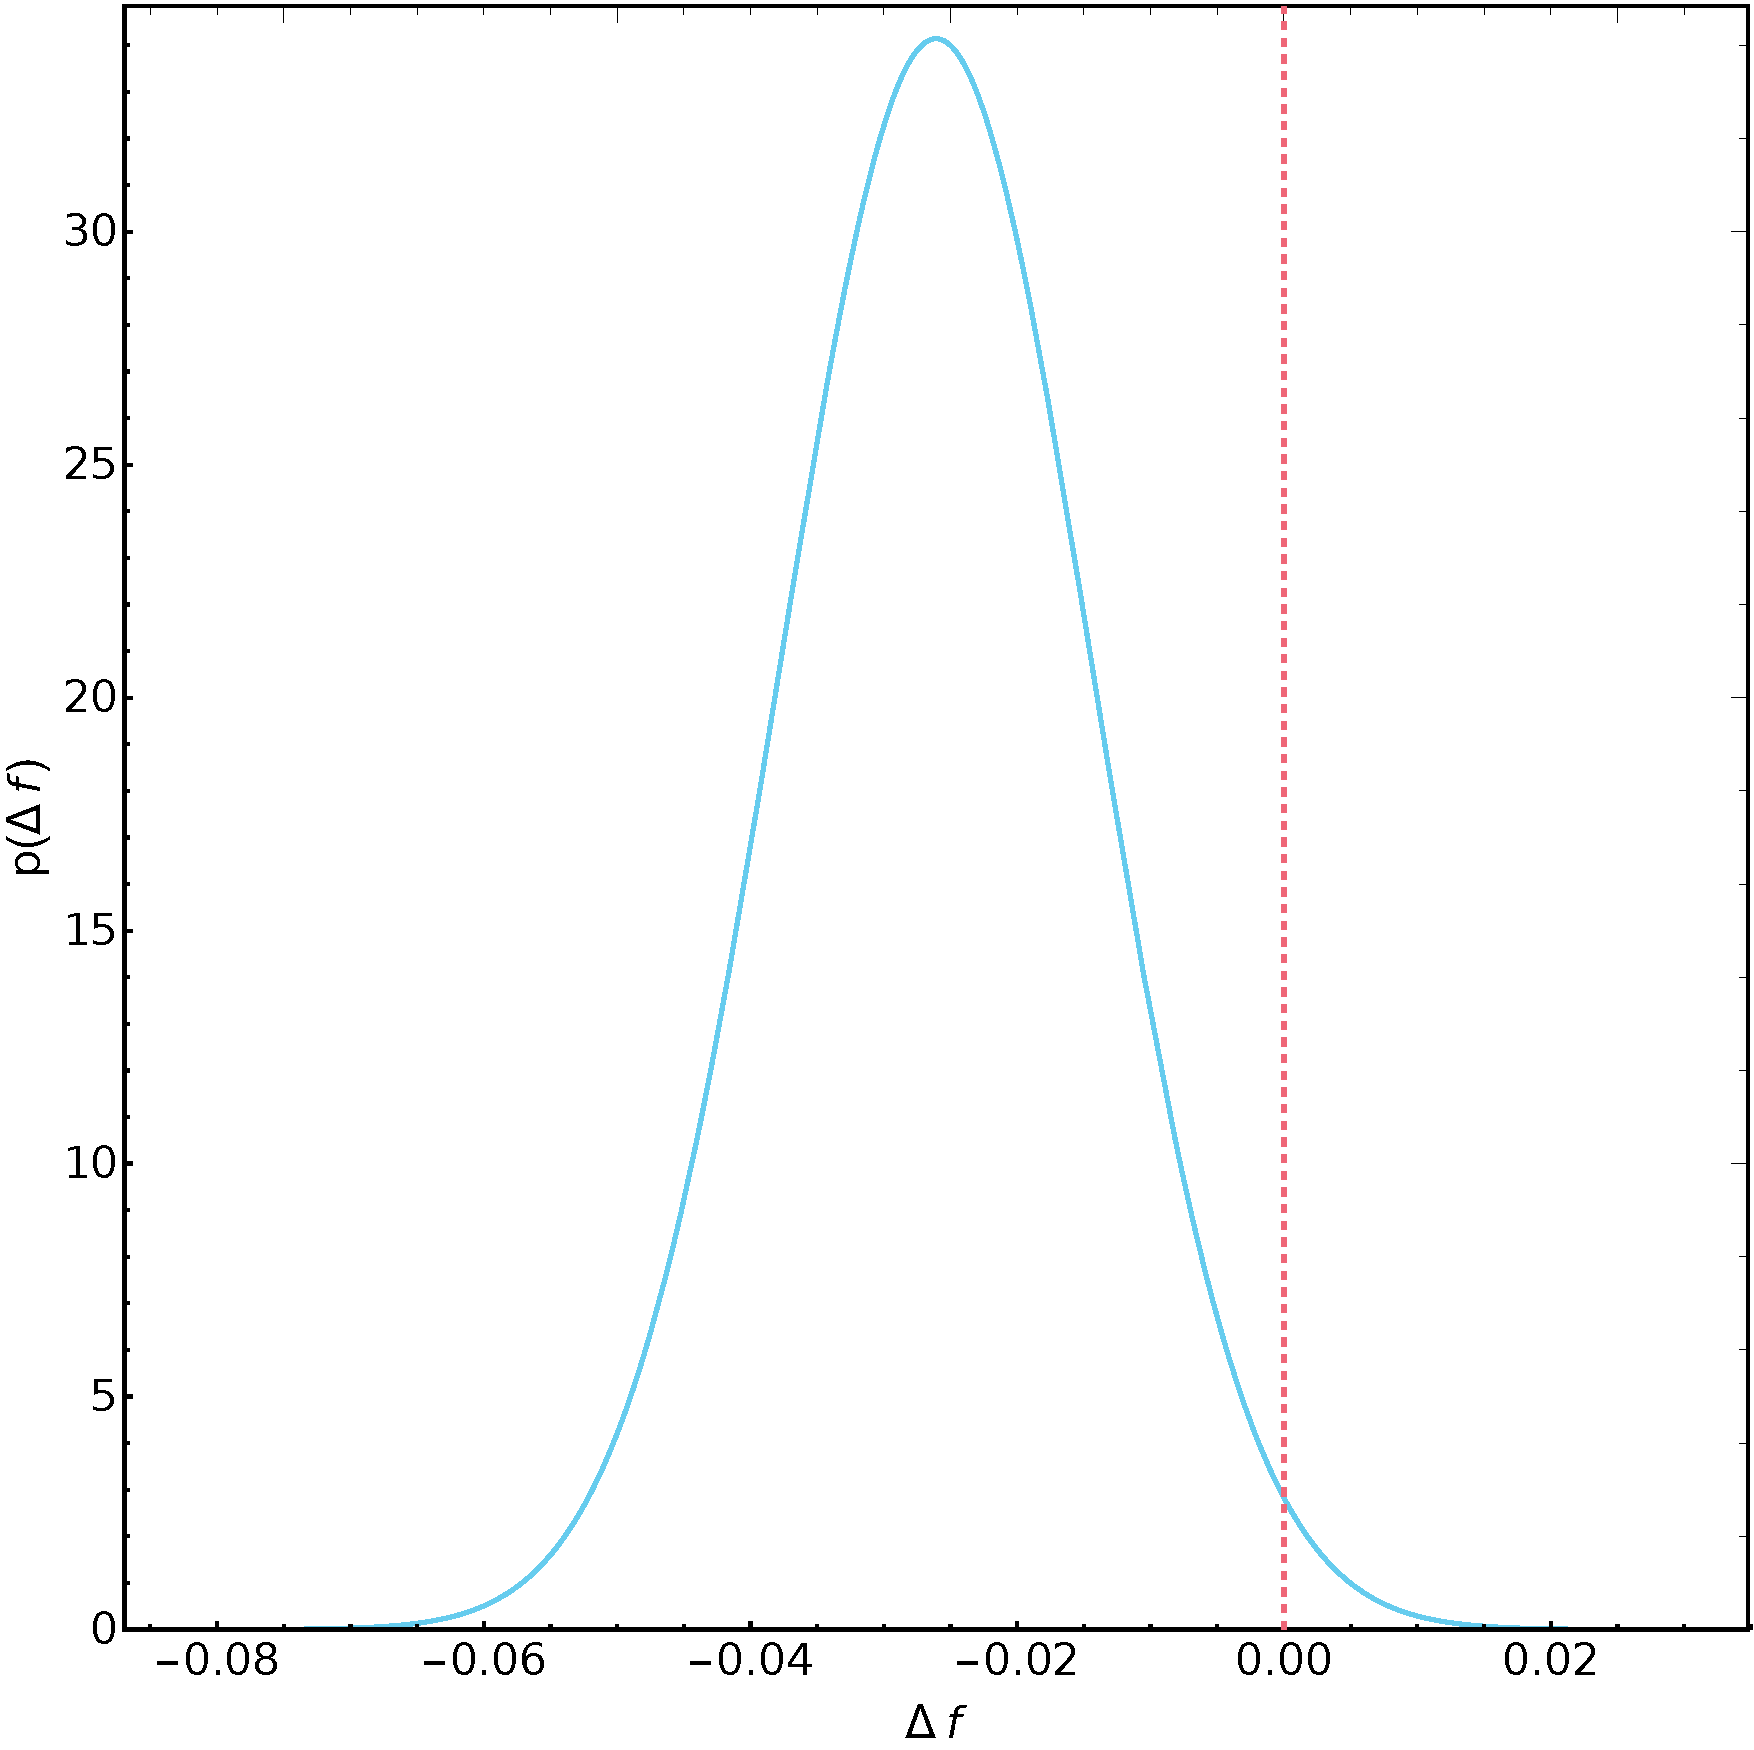
\includegraphics[width=0.75\linewidth]{example_diff.pdf}\\
 \caption{Example of uncertainty distribution about the conditional-frequency
   difference $\df$}\label{fig:example_difference_distributions}
\end{figure}% scripts2/plot_curves.nb
% freq-1_1_conserv-spreads-sym_O-snp_6-spr_2.233.csv
% "spread_y",-2.23267970003192
% "EV_y",-0.0260880661493155
% "SD_y",0.0116846434125515
This distribution gives us many pieces of information: for example, a
negative difference $\df$ is more plausible than a positive one; it is
8.3\% plausible that $\abs{\df}<0.01$, and therefore 91.7\% plausible that
$\abs{\df}>0.01$; it is 90\% plausible that $-0.045 < \df < -0.007$; and so
on. Several measures can be chosen to summarize the distribution with one
number. For example, we could use the plausibility that $\abs{\df}$ exceeds
a given value, say $\pf(\abs{\df} > 0.01)$. A roughly equivalent but
perhaps more preferable measure is the minimal frequency difference we are
highly sure about:
\begin{equation}\label{eq:significance_measure}
x\;\text{ such that }\; \pf(\abs{\df} > x)=0.9.
\end{equation}
For the plot of
\fig~\ref{fig:example_difference_distributions} such measure is $0.0112$.
\mynote{add something about dependence of broadness on sample size, and
  \enquote{smoothing} as discussed by MacKay \amp\ Bauman Peto
  \citey[\sect~2.6]{mackayetal1995}.}

A more complete quantification of our uncertainty is the distribution
$\pf(f_{|\ya}, f_{|\yb})$ among the possible joint values of the two
conditional frequencies, from which $\pf(\df)$ can be calculated. This
joint distribution is also the optimal starting point when frequencies
conditional on allele combinations of several \snp\ are considered. Our
goal is therefore to quantify this joint \dob, given:
\begin{enumerate*}[label=(\arabic*)]
\item the conditional frequencies in a population sample, \item our initial
  information or guesses about such frequencies.
\end{enumerate*} In formulae, we want to assign a numerical value to
\begin{equation}\label{eq:p_goal}
  \pf(\ptext{conditional frequencies} \|
  \ptext{sample data}, \ptext{initial information}).
\end{equation}
In the rest of this section we shall calculate this \dob\ by methodically
applying the probability calculus.

\medskip

First let's observe that the approach just outlined is not dichotomous,
unlike a classical significance test. We are not asking whether the
frequency difference is \enquote{significant} or not. Rather, we find a
gradation of cases: from conditional frequencies likely to be very
distinct, to conditional frequencies likely to be very similar. These cases
can be sorted, for example with the measure of
formula~\eqref{eq:significance_measure}, obtaining a sequence of \snp s
with a decreasing belief of causal association with the symptom. How many
of these \snp s are to be selected for further study depends on one's
experimental and computational resources.
\textcolor{white}{If you find this you can claim a postcard from us.}


% In the next sections we use formula~\eqref{eq:intuitive_Bayes} to estimate
% the limit frequencies given a sample of $6029$ individuals from \mynote{***
%   details here}. We shall first focus on the conditional frequencies of
% each insomnia symptom given one \snp\ at a time. The inferences in this
% case are very simple, intuitive, and easily visualizable. In the subsequent
% sections we shall consider the study of each symptom given \emph{pairs} of
% \snp s, and the study of all possible eight \emph{symptom combinations}
% given one \snp\ at a time.



\subsection{Inference: concrete calculation}
\label{sec:inference}

Once we know the quantity we want to quantify our uncertainty about, the
calculation of our \dobs\ follows almost mechanically from the rules of the
probability calculus
\citep{jeffreys1939_r1983,cox1946,jaynes1994_r2003,hailperin1996}. This
calculus also shows which \dobs\ we must provide at the start, to arrive at
the desired ones.

The first step is to use Bayes's theorem:
\begin{multline}
  \label{eq:intuitive_Bayes}
  \pf(\ptext{frequencies} \| \ptext{data}, \ptext{initial info})
  \propto{}\\
  \pf(\ptext{data} \| \ptext{frequencies}, \ptext{initial info})
  \times
  \pf(\ptext{frequencies} \| \ptext{initial info}),
\end{multline}
which says that we need to provide two kinds of \dob: the plausibility of
obtaining our sampled data if we had known the conditional frequencies in
the larger population; and our initial guess about the conditional
frequencies, before we observed the data. The first is given by a simple
sampling formula. The second can be modelled in several reasonable ways;
we'll see, however, that they all lead to very similar conclusions about
the conditional frequencies and their difference, owing to the large size
of our sample. Let's give explicit expressions for both.

First of all, introduce some notation. The conditional frequencies are
denoted $f_{|\ya}$, $f_{|\yb}$ as above. The data $\yD$ consist in the
conditional frequencies observed in the sample: $F_{|\ya}$ is the fraction
showing the symptom among the sampled individuals having allele $\ya$, and
$F_{|\yb}$ is the analogous fraction for allele $\yb$. Finally, our initial
information $\yI$ consists in our initial beliefs and in the numbers
$N_{\ya}$, $N_{\yb}$ of sampled individuals having allele $\ya$ and $\yb$;
although these numbers are part of $\yI$ we will sometimes write them
explicitly besides $\yI$. (Note that $N_{\ya}$, $N_{\yb}$ are not part of
the \enquote{data} in the sense that they don't help us to update our
belief about the frequencies $f_{|\ya}$, $f_{|\yb}$ and therefore remain on
the right side of the conditional.)

\iffalse
In this section we do step by step the calculations outlined above. For
definiteness we consider onset insomnia ($\ysS$) and the \snp\ rs875994
with alleles $\ya$, $\yb$. The limit conditional frequencies are denoted
$f_{\ya}$ and $f_{\yb}$. The sample data, denoted by $\yD$,
consist of the number of individuals $F_{\ya}$ that show symptom
$\ysS$ among the sampled individuals having allele $\ya$, and the number
$F_{\yb}$ showing the same symptom among those having allele $\yb$.
Our initial information consists in the number $N_{\ya}$ of sampled
individuals with allele $\ya$, and the number $N_{\yb}$ with allele $\yb$.
The total number of sampled individuals is therefore $N_{\ya}+N_{\yb}$.
This initial information and our initial beliefs are denoted by $\yI$; the
numbers $N_{\ya}$, $N_{\yb}$ will often be indicated explicitly even though
they're part of $\yI$.
\fi

With this notation, Bayes's theorem above is written
\begin{multline}
  \labelbis{eq:intuitive_Bayes}
  \pf(f_{|\ya}, f_{|\yb} \| \yD, \yI)
  \propto
  \pf(\yD \|f_{|\ya}, f_{|\yb}, \yI)\;
  \pf(f_{|\ya}, f_{|\yb} \| \yI)
  \equiv{}\\
  \pf(F_{|\ya}, F_{|\yb} \|f_{|\ya}, f_{|\yb}, N_{\ya},N_{\yb},\yI)\;
  \pf(f_{|\ya}, f_{|\yb} \| N_{\ya},N_{\yb},\yI).
\end{multline}

\medskip

\paragraph{Plausibility for the data given the frequencies}

Our \dob\ about the data given the frequencies is given by simple counting
and symmetry. We have an arbitrarily large population where a fraction
$f_{|\ya}$ of individuals having allele $\ya$ show the symptom, and a
fraction $1- f_{|\ya}$ therefore don't show the symptom. We casually
observe $N_{\ya}$ individuals with allele $\ya$. The plausibility that a
fraction $F_{|\ya}$ of these show the symptom is then counted as a
\enquote{drawing with replacement} (because of the arbitrarily large
size of the full population), given by a binomial distribution \cites[\chap~3]{jaynes1994_r2003}[\sect~4.6]{ross1976_r2010}[\sect~VI.2]{feller1950_r1968}:
\begin{equation}
  \label{eq:sampling_belief}
  \pf( F_{|\ya} \| f_{|\ya},  N_{\ya}, \yI)
  =
\binom{N_{\ya}}{N_{\ya}\,F_{|\ya}}\;  {f_{|\ya}}^{N_{\ya}\,F_{|\ya}} \;
  {(1-f_{|\ya})}^{N_{\ya}\,(1-F_{|\ya})}.
\end{equation}

An analogous reasoning holds for allele $\yb$. Our belief about obtaining
the data is therefore
\begin{equation}
  \label{eq:sampling_belief_combined}
  \pf(F_{|\ya},F_{|\yb} \|  f_{|\ya},f_{|\yb}, N_{\ya}, N_{\yb}, \yI)
  =
 \prod_{x=\ya,\yb} \binom{N_{x}}{N_{x}\,F_{|x}}\;{f_{|x}}^{N_{x}\,F_{|x}} \;
  {(1-f_{|x})}^{N_{x}\,(1-F_{|x})}.
\end{equation}

\medskip

\paragraph{Initial plausibility for the frequencies}

We consider two different initial assumptions about the conditional
frequencies. Their densities are represented in
\fig~\ref{fig:initial_beliefs}. The first (left plot) assigns equal
plausibility to equal areas in the $(f_{|\ya},f_{|\yb})$-coordinate plane;
we call this the \enquote{uniform} state of knowledge and denote it $\yIu$.
The second (right plot) expresses a strong belief that the two frequencies
should be equal, as clear from the steep density increase towards the diagonal of
the $(f_{|\ya},f_{|\yb})$-coordinate plane; we call this a
\enquote{conservative} state of knowledge and denote it $\yIc$.
\begin{figure}[b!]%{r}{0.4\linewidth} % with wrapfigure
 \centering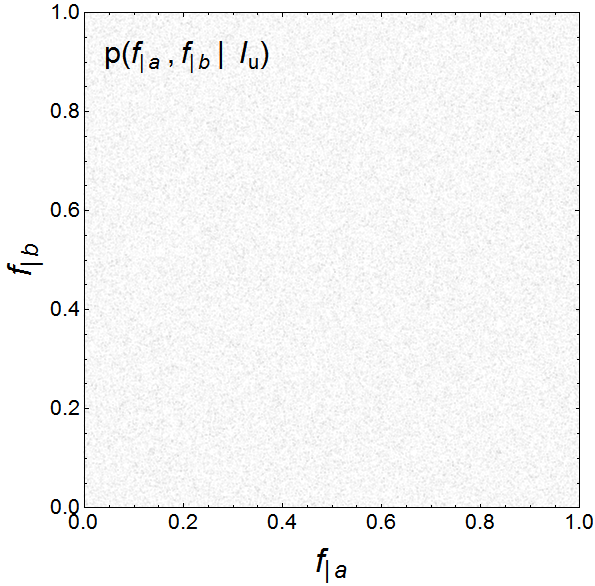
\includegraphics[width=0.49\linewidth]{unif_prior_list.png}%
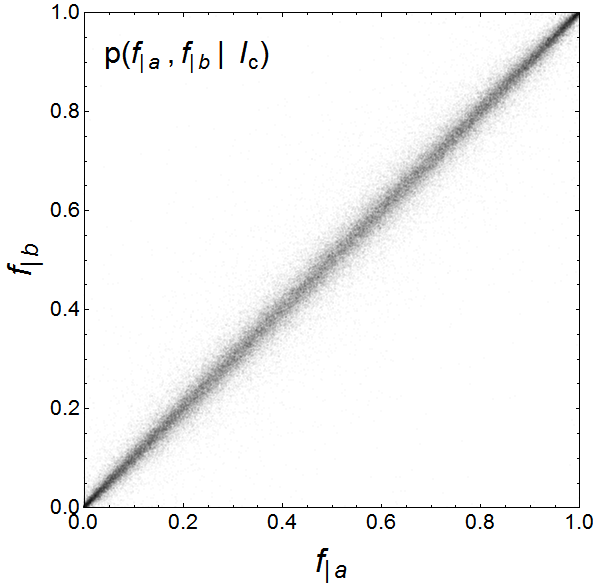
\includegraphics[width=0.49\linewidth]{conserv_prior_list.png}
\caption{Qualitative plot of our initial beliefs}\label{fig:initial_beliefs}
\end{figure}% scripts2/plot_priors.nb


The uniform state of knowledge is given by the simple density
\begin{equation}
  \label{eq:uniform_prior}
  \pf(f_{|\ya}, f_{|\yb} \| \yIu)%\;\di f_{|\ya}\,\di f_{|\yb}
  =1.%\di f_{|\ya}\,\di f_{|\yb}.
\end{equation}
The conservative state of knowledge is given by the following integral:
\begin{gather}
  \label{eq:conservative_prior}
  \pf(f_{|\ya}, f_{|\yb} \| \yIc)%\;\di f_{|\ya}\,\di f_{|\yb}
  =
  \int_{\mathrlap{0}}^{\mathrlap{\infty}}\di\yua
  \int_{\mathrlap{0}}^{\mathrlap{\infty}}\di\yub\;
\pf(f_{|\ya}, f_{|\yb} \| \yua,\yub,\yIc)\;
  \pf(\yua,\yub \| \yIc)%\;\di f_{|\ya}\,\di f_{|\yb}
  \\
\shortintertext{with}
  \label{eq:beta_product}
\pf(f_{|\ya}, f_{|\yb} \| \yua,\yub,\yI)\defd
  \dbeta(f_{|\ya} \| \yua,\yub)\;
  \dbeta(f_{|\yb} \| \yua,\yub),
  \\
  \pf(\yua,\yub \| \yIc)\defd \frac{1}{u+v}\,\dgamma(u+v \| 1, 1000)
\end{gather}
where $\dbeta$ and $dgamma$ are a beta and a gamma density:
\begin{gather}
  \label{eq:def_beta}
  \dbeta(f \| \yua,\yub) \defd
  \frac{\Gamma(\yua+\yub)}{\Gamma(\yua)\,\Gamma(\yub)}\;
  f^{\yua-1}\;(1-f)^{\yub-1},
  \qquad  \yua,\yub>0,
  \\
  \label{eq:def_gamma}
  \dgamma(\yA \| 1, 1000) \defd
  \frac{1}{1000}\,\exp(\yA/1000).
\end{gather}
The particular shape and scale values of the gamma density are chosen so as
to concentrate our initial belief along the $(f_{|\ya}, f_{|\yb})$
diagonal; this choice has also a deeper interpretation, discussed in
appendix***.


We express $\pf(f_{|\ya}, f_{\yb} \| \yI)$ as an integral to
emphasize that our initial beliefs about $f_{|\ya}$ and
$f_{\yb}$ are \emph{not} disjoint, and to show how their mutual
dependence comes about: by first considering two independent densities
having the same parameters, and then mixing their product over these
parameters.


We will examine how much our conclusions about the frequencies differ
between the two initial states of knowledge. Note that the second is indeed
very conservative. Therefore, if our updated belief conditional on the data
will show clearly distinct conditional frequencies, it will be because the
data have given enough evidence to overwhelm this conservative belief.




This construction has the interesting consequence for our updated belief
$\pf(f_{|\ya}, f_{\yb} \| \yD, \yI)$. According to Bayes's
theorem~\eqref{eq:intuitive_Bayes} combined with our initial
belief~\eqref{eq:beta_gamma_prior} it is given by
\begin{equation}
  \label{eq:straight_Bayes}
  \pf(f_{|\ya}, f_{\yb} \| \yD, \yI)
  \propto
  \pf(\yD \| f_{|\ya}, f_{\yb} \| \yI)\;
  \pf(f_{|\ya}, f_{\yb} \| \yI),
\end{equation}
but, as shown in appendix~\ref{sec:bayes_hierarcic}, it can also be written
in the following way:
\begin{equation}
  \label{eq:formal_hierarchic}
  \pf(f_{|\ya}, f_{\yb} \| \yD, \yI) =
  \tint\di\yua\tint\di\yub\;
  \pf(f_{|\ya}, f_{\yb}\| \yD,\yua,\yub,\yI)\;
  %   \dbeta(f_{|\ya} \| \yua,\yub)\,
  % \dbeta(f_{\yb} \| \yua,\yub)\;
  \dA(\yua,\yub \|\yD, \yI),
\end{equation}
with the normalized density $\dA(\yua,\yub \|\yD, \yI)$ defined by
\begin{multline}
  \label{eq:update_hyperparameter}
  \dA(\yua,\yub \|\yD, \yI) \propto   \dA(\yua,\yub \|\yI)
\times{}\\
%\Bigl[
\underbrace{\tint\di f_{|\ya}\tint\di f_{\yb}\;
  \pf(\yD \|f_{|\ya}, f_{\yb}, \yI)\;
 \pf(f_{|\ya}, f_{\yb} \|\yua,\yub, \yI)}_{\zerob{\footnotesize${}\defs\pf(\yD \|\yua,\yub,\yI)$}}.
      % \dbeta(f_{|\ya} \| \yua,\yub)\,
      % \dbeta(f_{\yb} \| \yua,\yub)
%       \Bigr]
\end{multline}
It is as if $\yua$, $\yub$ were unknown parameters with initial belief
density $\dA(\yua,\yub \|\yI)$, and our update for the frequencies proceeded by
first updating our belief about the parameters,
\eqn~\eqref{eq:update_hyperparameter}, and then marginalizing them out,
\eqn~\eqref{eq:formal_hierarchic}. This is a so-called \emph{hierarchic}
model \citep{good1980}. This hierarchic way of thinking often helps in
constructing densities that better represent our initial beliefs, and also
leads to formulae that can be better approximated when exact computation is
unfeasible. A point rarely emphasized in the literature, though, is that
there is no mathematical difference between a hierarchic and a
non-hierarchic model: we could forget about the integrals in
formula~\eqref{eq:beta_gamma_prior} and about the update
formula~\eqref{eq:formal_hierarchic}, and simply treat
$\pf(f_{|\ya}, f_{\yb} \| \yI)$ as the density depicted in
\fig~\ref{fig:initial_belief}, with update~\eqref{eq:intuitive_Bayes}. The
results would be the same. Further discussion about the formulae above is
given in \sect***.


With large sample sizes the density $\dA(\yua,\yub \|\yD, \yI)$ turns out to
be so peaked with respect to
$\pf(f_{|\ya}, f_{\yb}\| \yua,\yub,\yI)$ that it can be considered
as a Dirac delta centred on the parameters $\yuam$, $\yubm$ that maximize it.
We thus obtain a good approximation of the updated
belief~\eqref{eq:formal_hierarchic} that doesn't involve parameter integration:
\begin{multline}
  \label{eq:formal_hierarchic_approx}
  \pf(f_{|\ya}, f_{\yb} \| \yD, \yI) \approx
  \pf(f_{|\ya}, f_{\yb}\| \yuam,\yubm,\yI)\\
  \text{with}\quad
  (\yuam,\yubm) \defd \argmax_{\yua,\yub}\dA(\yua,\yub \|\yD, \yI).
\end{multline}
The maximum of $\dA(\yua,\yub \|\yD, \yI)$, or better of its logarithm, can
easily be found with most optimization methods. The explicit expression to
be optimized, discussed in appendix***,
\begin{equation}
  \label{eq:to_optimize}
  \yna\,[\ln\Gamma(\tsum_s\yu_s) - \tsum_s\ln\Gamma(\yu_s)]
  -\sum_{\mathclap{x=\ya,\yb}}
  [\ln\Gamma(N_x+\tsum_s\yu_s) - \tsum_s\ln\Gamma(N_xF_{s\|x}+\yu_s)]
\end{equation}

Combininig \eqns~\eqref{eq:formal_hierarchic_approx},
\eqref{eq:def_ff_given_Aq}, \eqref{eq:def_beta} we thus arrive at the
following explicit approximate formula for our belief about the conditional
frequencies given the data:
\begin{multline}
  \label{eq:formal_hierarchic_approx_final}
  \pf(f_{|\ya}, f_{\yb} \| \yD, \yI) \approx
  \dbeta(f_{|\ya} \| \yuam,\yubm)\;
  \dbeta(f_{\yb} \| \yuam,\yubm)\\
  \text{with
    $(\yuam,\yubm)$ maximizing~\eqref{eq:to_optimize}}.
\end{multline}




 \mynote{ref here to \citep{mackay1996}}
\subsection{Generalization to symptom combinations}
\label{sec:generalization_symptom_combinations}




\subsection{Choices of initial beliefs and meaning of the parameters}
\label{sec:choices_prior_info}


The parameters $\yu$ of the Dirichlet density for the frequency
distribution $\yf$ have very intuitive meanings, even more evident if we
rewrite them as their sum and a pair of normalized parameters:
\begin{equation}
  \label{eq:rewrite_params}
  \yA \defd \ysum\yu,
  \qquad
  \yq\defd\yu/\sum\yu.
\end{equation}
The normalized parameters $\yq$ are the expected frequency distribution:
\begin{equation}
  \label{eq:meaning_normalized_parameters}
  \expe{\yf \| \yu} = \yq
\end{equation}
The sum of the parameters $\yA$ expresses the sharpness of the
distribution, as seen from the covariance matrix:
\begin{equation}
  \label{eq:variances_covariances}
  \var(f_i \| \yu) = \frac{\yqq_i\;(1-\yqq_i)}{\yA+1},
  \qquad
  \cov(f_i\,f_j \| \yu) = -\frac{\yqq_i\,\yqq_j}{\yA+1}.
\end{equation}
In fact, from the update formula*** we see that $\yA$ quantifies the amount
of data necessary to modify our initial belief.



\[
  \frac{  \expe{f_{\ysA\|\ya} - f_{\ysA\|\yb} \| \yD, \yI}}{
    \std(f_{\ysA\|\ya} - f_{\ysA\|\yb} \| \yD, \yI)}
\]


\section{Results}
\label{sec:results}



\begin{figure}[b!]%{r}{0.4\linewidth} % with wrapfigure
 \centering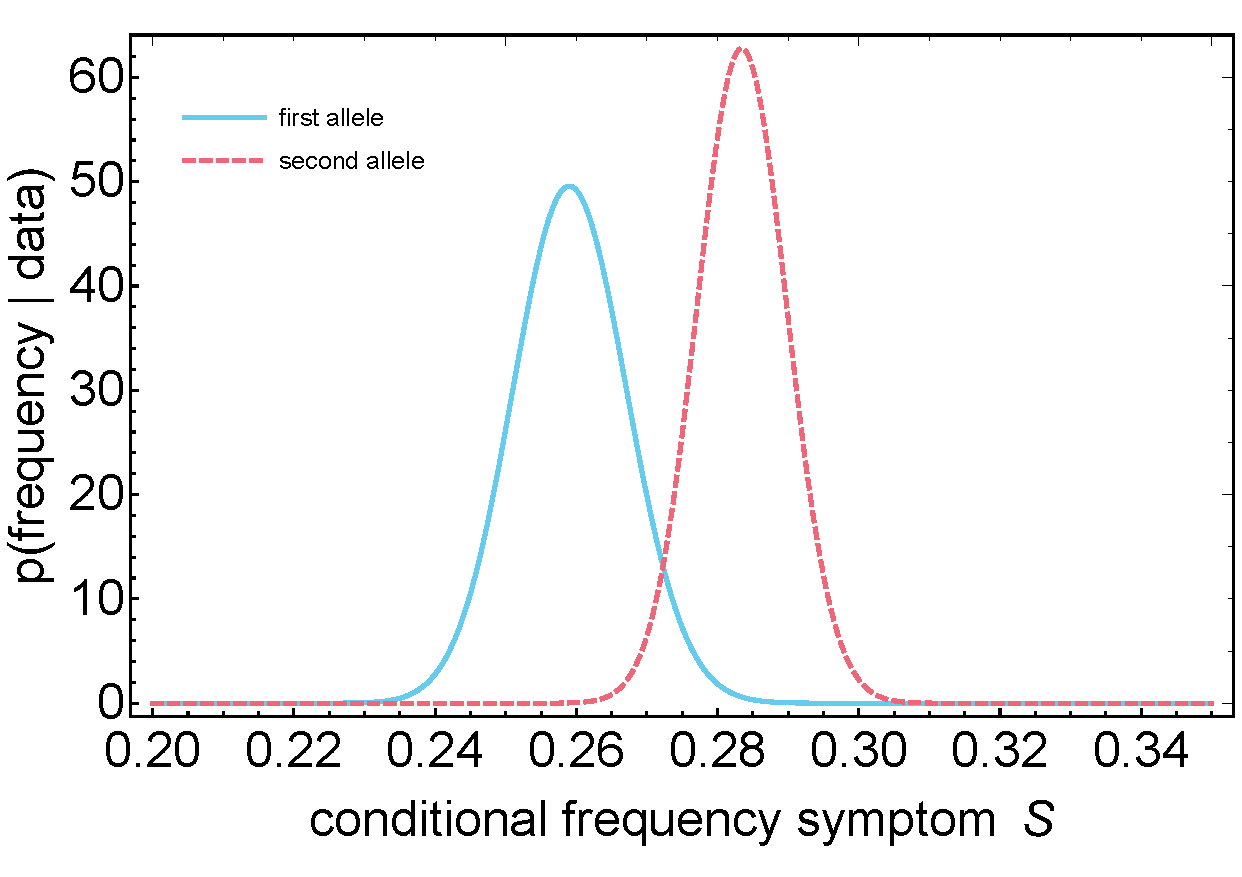
\includegraphics[width=0.75\linewidth]{example_distr_condfreqs.pdf}\\
\caption{Example of distributions of belief}\label{fig:example_distributions}
\end{figure}% scripts/single_gene_condfreqs_thetamax.nb
%% EVs: 0.25917, 0.283506; SDs: 0.00804727, 0.00635616
%% overlap at 0.01 = 0.0321908



\begin{figure}[b!]%{r}{0.4\linewidth} % with wrapfigure
 \centering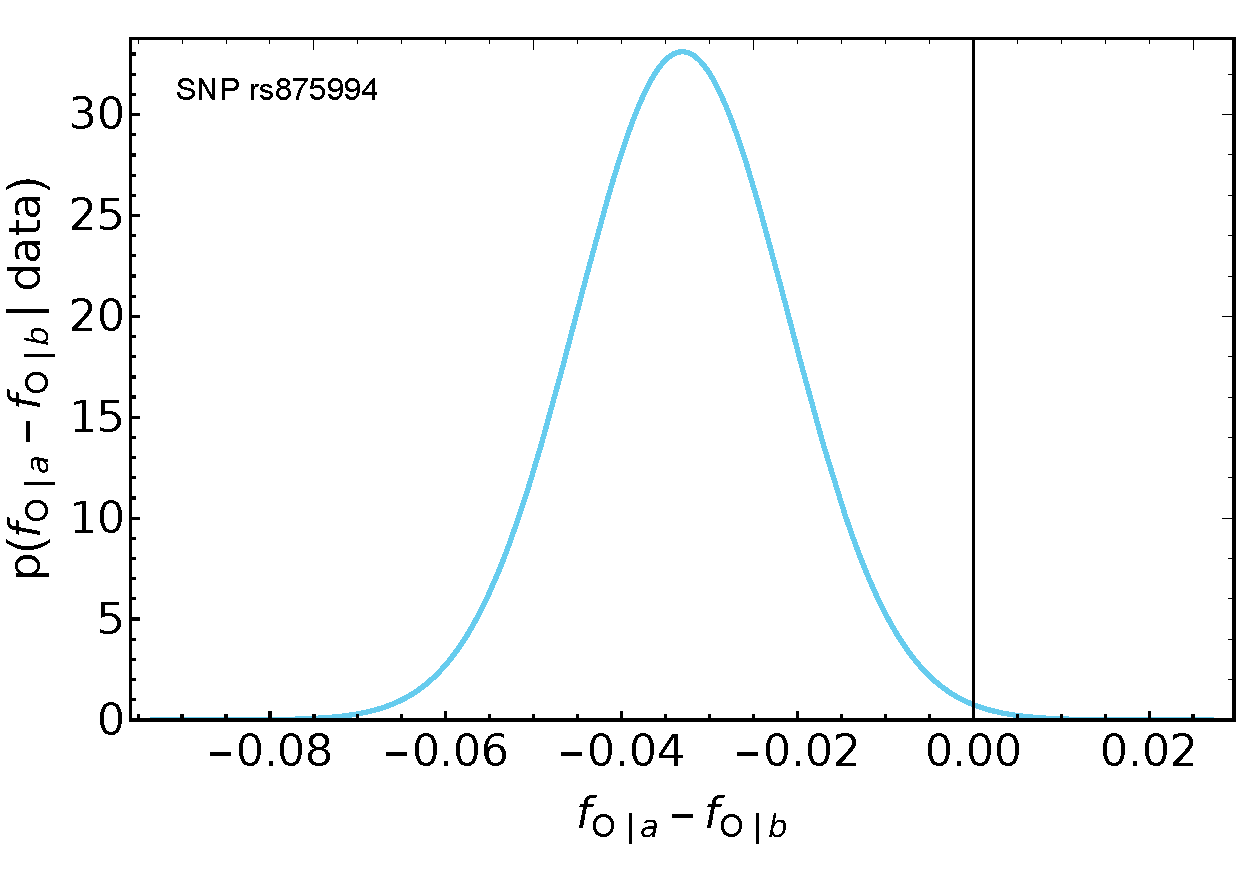
\includegraphics[width=0.75\linewidth]{difference_symA_snp6.pdf}\\
 \caption{Distribution for the difference between the frequencies
   $f_{\ysA\|\ya}$, $f_{\ysA\|\yb}$ of onset insomnia ($\ysA$) conditional on
   the two alleles of \snp\ rs875994}\label{fig:difference_distributions}
\end{figure}% scripts/condfreqs_general_tests.nb
%% snp #6,
%% EV: -0.0330998, SD: 0.0120472
%% EV/SD: 2.75
%% 0.0274176 within 0.01

\newpage
%\renewcommand*{\appendixpagename}{Appendix}
%\renewcommand*{\appendixname}{Appendix}
%\appendixpage
\appendix


\section{Derivation of Bayes's theorem in hierarcic form}
\label{sec:bayes_hierarcic}

We write Bayes's theorem~\eqref{eq:straight_Bayes} with our initial
belief~\eqref{eq:beta_gamma_prior} written in full:
\begin{equation}
  \label{eq:straight_Bayes_full_prior}
  \pf(f_{\ysA\|\ya}, f_{\ysA\|\yb} \| \yD, \yI)
  \propto
  \tint\di\yA\tint\di\yq\;
    \pf(\yD \| f_{\ysA\|\ya}, f_{\ysA\|\yb} \| \yI)\;
 \pf(f_{\ysA\|\ya}, f_{\ysA\|\yb} \|\yA,\yq, \yI)\;
  \dA(\yA,\yq \|\yI).
\end{equation}
Multiplying and dividing within the integral with the expression
\begin{equation}
  \label{eq:def_Aq_given_data}
    \pf(\yD \|\yA,\yq,\yI)\defd
\tint\di f_{\ysA\|\ya}\tint\di f_{\ysA\|\yb}\;
  \pf(\yD \|f_{\ysA\|\ya}, f_{\ysA\|\yb}, \yI)\;
  \pf(f_{\ysA\|\ya}, f_{\ysA\|\yb}\| \yA,\yq,\yI)
      % \dbeta(f_{\ysA\|\ya} \| \yA,\yq)\,
      % \dbeta(f_{\ysA\|\yb} \| \yA,\yq)
\end{equation}
we obtain the alternative form~\eqref{eq:formal_hierarchic}



Combining together the sampling
formula~\eqref{eq:sampling_belief_combined}, the expression of the beta
density~\eqref{eq:def_beta}, and the update
formula~\eqref{eq:update_hyperparameter} we obtain
\begin{multline}
  \label{eq:parameter_posterior_first}
  \dA(\yA,\yq \|\yD, \yI) \propto
    \dA(\yA,\yq) \times{}\\
  \Bigl[   \tint\di f_{\ysA\|\ya}\tint\di f_{\ysA\|\yb}\;
  \dbeta\Bigl(f_{\ysA\|\ya} \bigcond \yA+N_{\ya},
  \frac{\yA\yq+N_{\ya}F_{\ysA\|\ya}}{\yA+N_{\ya}}
    \Bigl)\;
  \dbeta\Bigl(f_{\ysA\|\yb} \bigcond \yA+N_{\yb},
  \frac{\yA\yq+N_{\yb}F_{\ysA\|\yb}}{\yA+N_{\yb}}
    \Bigr)
       \Bigr]
%  \pf(f_{\ysA\|\ya}, f_{\ysA\|\yb} \|\yA,\yq, \yI)\;
\end{multline}


\section{Summary of the main formulae}

We have a sample of size $n$. We check the subsample of individuals that
have a particular allele, say Bx, for a particular gene, say rs697680\_A.
Suppose that in this subsample $n_0$ individuals \emph{don't} show symptom
A and $n_1$ \emph{do} show symptom A. This also means that the size of our
subsample (individuals with allele Bx) is $n \defd n_0+n_1$.

Our \dob\ about the frequency $f_1$ of symptom A among the individuals with
allele Bx in an \emph{infinite} population is a Beta distribution with
parameters $n_0+\theta_0$, $n_1+\theta_1$, with
$\theta \defd \theta_0+\theta_1$:
\begin{multline}
  \label{eq:beta_fr}
  \pf(f_1 \| n_0,n_1,\theta_0,\theta_1)\;\di f_1 ={}\\
  \frac{\Gamma(n+\theta)}{\Gamma(n_0+\theta_0)\;\Gamma(n_1+\theta_1)}
  \; (1-f_1)^{n_0+\theta_0-1}\;{f_1}^{n_1+\theta_1-1} \;\di f_1
\end{multline}
This distribution has expected value and variance
\begin{equation}
  \label{eq:exp_value}
  \begin{split}
  \expe{f_1 \| n_0, n_1, \theta_0,\theta_1} &= \frac{n_1+\theta_1}{n+\theta},
  \\
  \var(f_1 \|  n_0, n_1, \theta_0,\theta_1) &=
  \frac{(n_0+\theta_0)\;(n_1+\theta_1)}{(n+\theta)^2\;(n+\theta+1)}.
\end{split}
\end{equation}



\mynote{Possible further developments: use of hyper-Dirichlet priors, use
  of graphical models to infer causal relationships
  \citep{pearl2000_r2009}}

\[
\begin{aligned}
\pf(f \|\yD)  &\propto \pf(\yD \| f)\;\pf(f \| \yI)
  \\
  &\propto \pf(\yD \| f)\;\int\di u\, \pf(f \|u)\, \pf(u\| \yI)
  \\
  &\propto \int\di u\,\pf(\yD \| f)\; \pf(f \|u)\; \pf(u\| \yI)
  \\
  &\propto \int\di u\,\pf(\yD \| f,u)\, \pf(f \|u)\;
    \pf(\yD \| u)\, \pf(u\| \yI)
  \\
  &\propto \int\di u\,\pf(f \| D,u)\;
    \pf(u \| \yD)
\end{aligned}
\]

\[
  \begin{aligned}
    \pf(u \|\yD)
    &\propto \int\di f\, \pf(\yD \| f)\,\pf(f \| u)\;\pf(u \| \yI)
    \\
    &\propto
      \prod_{x=\ya,\yb}\Biggl[ 
      \frac{\Gamma(\tsum_su_s)}
      {\tprod_s\Gamma(u_s)}\;
      \frac{\tprod_s\Gamma(N_xF_{s\|x}+u_s)}
      {\Gamma(N_x+\tsum_su_s)}
       \Biggr]
  \end{aligned}
\]


\[
  \pf(f_{\ysA\|\ya}, f_{\ysA\|\yb} \| \yD, \yI) \approx
  \pf(f_{\ysA\|\ya}, f_{\ysA\|\yb}\| \yuam,\yubm,\yI)
\]



%

%\setlength{\intextsep}{0.5ex}% with wrapfigure
%\begin{figure}[p!]%{r}{0.4\linewidth} % with wrapfigure
%  \centering\includegraphics[trim={12ex 0 18ex 0},clip,width=\linewidth]{maxent_saddle.png}\\
%\caption{***}\label{fig:comparison_a5}
%\end{figure}% exp_family_maxent.nb

%\newpage

\begin{acknowledgements}
  PGLPM thanks Mari \amp\ Miri for continuous encouragement and affection, and
  to Buster Keaton and Saitama for filling life with awe and inspiration.
  To the developers and maintainers of \LaTeX, Emacs, AUC\TeX, Open Science
  Framework, Python, Inkscape, Sci-Hub for making a free and unfiltered
  scientific exchange possible.
%\rotatebox{15}{P}\rotatebox{5}{I}\rotatebox{-10}{P}\rotatebox{10}{\reflectbox{P}}\rotatebox{-5}{O}.
%\sourceatright{\autanet}
\end{acknowledgements}



%%%%%%%%%%%%%%% BIB %%%%%%%%%%%%%%%

\defbibnote{prenote}{{\footnotesize (\enquote{de $X$} is listed under D,
    \enquote{van $X$} under V, and so on, regardless of national
    conventions.)\par}}
% \defbibnote{postnote}{\par\medskip\noindent{\footnotesize% Note:
%     \arxivp \mparcp \philscip \biorxivp}}

\printbibliography[prenote=prenote%,postnote=postnote
]


\end{document}


%%% Local Variables: 
%%% mode: LaTeX
%%% TeX-PDF-mode: t
%%% TeX-master: t
%%% End: 
